\documentclass[a4paper,12pt]{report}

%do wstawiania obrazków
\usepackage{graphicx}

%adresy URL
\usepackage{url}

%zakladki w pdf:
\usepackage[pdftex,bookmarks=true,colorlinks=true,linkcolor=black,urlcolor=black,citecolor=black]{hyperref}

% ustawienia strony 
% przeczytac plik w:
% D:\Projekty\Bachelor\info\wytyczneMagInz.pdf
% ustawienie marginesów
\oddsidemargin = 10pt
\textwidth = 450pt

\usepackage{color}
\usepackage[scriptsize,bf]{caption}
\usepackage{pdfpages}

%listing kodu
\usepackage{listings}
\definecolor{darkgray}{rgb}{0.95,0.95,0.95}
\lstset{ %
        language=Java,                % the language of the code
        basicstyle=\scriptsize,       % the size of the fonts that are used for the code
        numbers=left,                   % where to put the line-numbers
        numberstyle=\tiny,      % the size of the fonts that are used for the line-numbers
        numbersep=10pt,                  % how far the line-numbers are from the code
        showspaces=false,               % show spaces adding particular underscores
        showstringspaces=false,         % underline spaces within strings
        showtabs=false,                 % show tabs within strings adding particular underscores
        tabsize=2,                      % sets default tabsize to 2 spaces
        captionpos=b,                   % sets the caption-position to bottom
        breaklines=true,                % sets automatic line breaking
        breakatwhitespace=false,        % sets if automatic breaks should only happen at whitespace
        backgroundcolor=\color{darkgray},
        xleftmargin=35pt}


%nagłówek i stopka
\usepackage{fancyhdr}

\pagestyle{fancyplain}
%\renewcommand{\chaptermark}[1]{\markboth{#1}{}}
\renewcommand{\chaptermark}[1]{\markboth{\chaptername\ \thechapter.\ #1}{}}

\lhead{}
\chead{}
\rhead{\fancyplain{}{\textit{\leftmark}}}
\lfoot{}
\cfoot{\thepage}
\rfoot{}

%1,5 linii odstępu
\linespread{1,3}

\setlength{\parindent}{0mm} % ustawi rozmiar wciecia na poczatku kazdego akapitu na 0mm,
\setlength{\parskip}{4mm} %ustawi rozmiar odstepu pomiedzy kolejnymi akapitami na 4mm,

%numerowanie definicji
        \newtheorem {definition}{Definition}[chapter]%[section]
%numerowanie przykladow
        \newtheorem {example}{Example}[chapter]%[section]

%info dla pliku pdf
\pdfinfo{
   /Author (Zbyszko Natkanski)
   /Title  (Software Metrics for Predicting Faults)
   /Subject (Software Metrics for Predicting Faults)
   /Keywords (Master thesis, MSc, Master)
}

\usepackage{acronym}
%\usepackage{rotating} 
 
 
%=======[BEGIN DOCUMENT]===========
\begin{document}

%========[!!!!!!!!!!!!!!!] ============> strona tytułowa [UNCOMMENT!]

\includepdf[pages={1}]{title-page-beta.pdf}

%spis tresci
\tableofcontents       
%------------------------------------------------------------

\newpage
\phantomsection \label{bib}
\addcontentsline{toc}{chapter}{Abstract}
\chapter*{Abstract}
\label{roz:abstract}

This thesis presents the overview of software metrics, implementing them tools and shows the practical usage of metrics in casual project. Nowadays, metrics could be treated as fundamental determinants of software quality which is essential in providing software product free from faults. What is more, the last decades show that a quality analysis attracts a lot of attention among researchers and developers.

The review of tools implementing software metrics enables to choose the best tools adjusted to each software engineering project. 
 
In order to prove practical usage, the exemplary academic project were taken into consideration. The measurement made with use of metrics plug-ins for Eclipse IDE enable to derive the conclusions indicating area of improvements that project need. 

This thesis categorizes and summarizes also the existing metrics, so it could be applied as supportable guide for developers and project managers. 


%introduction - teza, cel i zakres pracy
\chapter{Introduction} \label{roz:wstep}
Nowadays, the software engineering is very intellectual process, because of its dynamic and unpredictable environment. Keeping the software quality requires to determine the measurements methods that will describe what the quality is and how it could be tracked.  The instant growth of software industry realized the customers how valuable are provided products. What is more, customers are aware of breaking next technological barriers, so they are not willing to compromise of quality aspects. That is way, the software metrics are the first indicators of design or code quality.
 
Another important aspect of software metrics is fact that the maintenance and evolution of software systems are major issue in industry. Within the time, most of the systems tend to decay in quality if they are not adapted to changing requirements and standards. So it is necessary to have a possibility to track the system quality within the time. It is a time and money saving approach for complex systems, because metrics are treated as \textit{tool} for attaining accurate estimation of project milestones and develop a system with minimal number of faults. 
 
In order to facilitate the quality of software a large set of metrics have been developed and many tools exist to collect metrics from code or design representation. It allows users to select the best tool to support and handling projects.

\section{Purpose}
The purposes of this thesis are:

\begin{itemize}
\item to review and classify software metrics basing on professional literature, academic publications and results of research made by software development teams, 
\item to identify areas of software engineering process enabling to use and apply a software metrics,
\item to review tools that implements software metrics for Java language,
\item practical usage of software metrics and tools implementing metrics that indicate areas that need to be improved, 
\item final evaluation of usefulness of software metrics in software engineering. 
\end{itemize}

\section{Range of thesis}
The particular chapters of thesis contain:

\begin{itemize}
\item Chapter~\ref{roz:basic_terms} describes the basic terms that are used in the thesis. There are given definitions of software metrics, object--oriented terms and graph theory. It enables not advanced readers to get familiar with research area. 
\item The theoretical approach to software metrics is described in Chapter~\ref{roz:metrics_theory}. It explains the reason of making measurements and introduces Software Quality Model with set of commonly used software metrics. The following sections represent the groups in which the metrics have been divided and assigned. 
\item Chapter~\ref{roz:metrics-tools} focuses on tools (plug-ins) that implements software metrics. In the summary, it is attempt to indicate the best tools to use during software project development. 
\item Basing on one of the academical project, tools introduces in previous chapter and explained software metrics, the practical approach to software metrics is made in Chapter~\ref{roz:metrics-practic}. The purpose is to analyse arbitrary project and indicate the aspects that need improvements. 
\item The final conclusions of whole thesis and further research development are described in Chapter~\ref{roz:conclusion}.  
\item The rest of chapters are bibliography and tables, figures and acronyms lists.
\end{itemize}
%------------------------------------------------------------

%basic terms
\chapter{Basic terms} \label{roz:basic_terms}

\textit{This chapter introduces and explains the basic terms that have been used in the thesis.}

\subsection*{Software metrics}
Software metrics are special kind of measurements specified for software used to identify quality of code, the complexity of the system and cost of maintenance and flexibility. The purpose of software metrics is to investigate and evaluate the quality of provided software and encourage developers to improve the quality of provided products~\cite{metrics}.

\subsection*{Software engineering}
Software engineering provides the theoretical foundations for building software and focuses on implementing the software in a controlled and scientific way.  It describes the collection of techniques that apply an engineering approach to the implement and support of software products. Software engineering activities include managing, costing, planning, modelling, analysing, specifying,  designing, implementing, testing, and maintaining. Engineering approach means that each activity is understood and controlled, so that there could be no surprises as the software is specified, designed, built, and maintained \cite{rigorous}.

\subsection*{Object-oriented metrics}
The rise in popularity of object oriented programming create a need to prepare metrics that are able to measure and evaluate aspects characteristic for objectivity: inheritance, polymorphism, encapsulation, cohesion and coupling. First set of object-oriented metrics were proposed by S.R. Chidamber and C.F. Kemerer~\cite{alain}.

\subsection*{Object-oriented programming paradigm}
Object-oriented programming paradigm is a concept of objects that have attributes (fields) and associated behaviour (procedures, methods, functions). Generally, the object is a instance of class. Class is a representation of abstraction and its instances are used to interact with each other. Nowadays, the most popular object-oriented programming languages are C++, Java, C Sharp  and Objective-C.  

\begin{quote}
\textit{Object-oriented programming is a method of implementation in which programs are organized as cooperative collections of objects, each of which represents an instance of some class, and whose classes are all members of a hierarchy of classes united via inheritance relationships} \cite{booch}.
\end{quote}

Object-oriented programming makes code easier to organize, understand and managed. The modification of code could be applied without affecting other aspect of system. It is easier to introduce update and upgrades and when the system grows over the years it is more manageable. It allows also to split the responsibility of functionality of code by several developers, so they could work individually for one system but for another components of this system~\cite{booch}.  

\subsection*{Inheritance}
Inheritance is a relation between classes where one class (called child, derived or subclass)  is extended by another class (called parent, base  or super class). This relationship rises a hierarchy where subclasses could inherit attributes and behaviours (methods) from pre-existing classes. The semantics of class inheritance could vary from language to language, but commonly the subclass automatically inherits the instance variables and member functions of its superclass. Some languages enable to inherit from many classes and the access to attributes and methods from parent class are defined by set of access modifiers (for example in Java language are public, private, protected and default modifiers).  The superclass defines a common interface and foundational functionality, which specialized subclasses could inherit, modify, and implement. The methods and attributes inherited by a subclass could be reused in the subclass. A reference to an instance of a class might be referring one of its subclasses. The actual class of the object being referenced is impossible to predict at compile-time. A uniform interface is used to invoke the member functions of objects of a number of different classes. Subclass might replace superclass functions with entirely new functions by naming its method the same as methods in super class (it is called overriding).  In some languages a class could be defined as unable to be inherited by adding to class special declaration (for Java it is a \textit{``final''} keyword and \textit{``sealed"} for C Sharp) Such word added to declaration of class restricts the re-usability of all methods and attributes of this class. Similar functionality could be also applied to some attributes or methods  from given class. 
Introducing inheritance mechanism enabled to limit number of duplicated code and separate behaviours from super class and enable to detail it in subclass~\cite{SCJP}.

\subsection*{Polymorphism}
Polymorphism refer to the biological principle in which organism or species could have different forms or stages. This principle has also its use in object oriented programming. Subclass of parent class can define their own unique behaviours (methods) and what is more, share the same of functionality of the parent class~\cite{JavaDoc}.

There are different kinds of polymorphism:
\begin{itemize}
\item \textit{``ad hoc'' polymorphism} is supported by many languages as function overloading and it means that method could be applied to arguments of different types.
\item \textit{parametric polymorphism} is marked when code is written without mentioned of any specific type and thus could be use with any number of types.
\item\textit{inclusion polymorphism (sub typing)} is a concept where a name might denote instances of many different classes as long as they are related by some common superclass~\cite{booch}.
\end{itemize}

General, polymorphism could refer to \textit{``many shapes''}. It is means ability to request the same operations, but performed by a wide range of different types of things. In OOP, the polymorphisms is achieved by using many different techniques named method overloading, operator overloading and method overriding.

\subsection*{Encapsulation}
Encapsulation is a mechanism for restricting access to some of object`s methods and attributes. It \textit{``is the process of compartmentalizing the elements of an abstraction that constitute
its structure and behaviour; encapsulation serves to separate the contractual interface of an
abstraction and its implementation''}~\cite{booch}.
This mechanism provides explicit kind of barrier which leads to a clear separation of access and non-accessible part of implementation. In practise it means that class should have two parts: an interface and implementation. The interface of the class presents only scheme, layout or list of instance of class behaviour. The implementation asserts the mechanism that allows realization of class behaviour. 

Another important assumption of encapsulation is hiding class arguments. It is realised by forbidding direct access to class`s arguments (using access modifiers) and providing methods allowing setting and getting its values. It prevents unauthorized parties direct access to them~\cite{SCJP}.

\subsection*{Coupling}
Coupling is the measure of the strength of association established by a connection from one class to another class. Strong coupling complicates a system because system is harder to understand, revise, change, or correct. This complexity could be reduced by designing system with weak dependency between classes.   

Coupling is the term borrowed from structural programming but is also applicable to object-oriented analysis and design. However the concepts of coupling does not refer to inheritance, (inheritance is in certain sense a type of coupling) because introduces significant improvement of presenting classification abstractions and dependencies in object oriented paradigm~\cite{booch}.

\subsection*{Cohesion}
The idea of cohesion is also taken from structural programming. Cohesion measures the degree of connection between objects in a single component. The one form of cohesion is coincidental cohesion where entirely unrelated abstractions are thrown into the same class, package or component. Another form of cohesion is functional cohesion. Elements of a class or component work together to provide some well-bounded behaviour~\cite{booch}.

\subsection*{Artefacts} 
Artefacts are used as the simplest form of measurement of source code. As the artefact it could be treated line(s) of code, field(s) of code, methods, classes, interfaces, components, packages. Basing on such artefacts, the quality of system could be evaluated. 

\subsection*{Graph theory}\label{section:graph_theory}
\subsubsection*{Simple graph}
A simple graph G is defined as a pair of sets (V, E), where:
\begin{itemize}\addtolength{\itemsep}{-0.5\baselineskip}\vspace{-7mm}
\item V is a finite non empty set of vertices, and
\item E is a set of pairs of vertices, called edges. 
\end{itemize}\vspace{-5mm}
It is often represented by $G = (V, E)$~\cite{graph}.

\subsubsection*{Chain}
In a simple graph $G = (V, E)$, a chain c is a finite sequence of vertices: $v_{0}, v_{1}, \cdots , v_{m}$ such that, for all i with $0 \textless= i \textless m, v_{i}, v_{i + 1}$ is an element of $E$.
\begin{itemize}\addtolength{\itemsep}{-0.5\baselineskip}\vspace{-7mm}
\item chain is represented by $c = [v_{0}, v_{1}, \cdots , x_{m}]$.
\item length of the path $c$ is the integer $m$, and it is represented by $l = m(c)$ (\cite{alain}).
\end{itemize}

\subsubsection*{Connected graph}
A graph G is connected if, for all x and for all y [vertices], there exists a chain connecting x and y.  A graph that is not connected could be divided into connected components.

\begin{itemize}\addtolength{\itemsep}{-0.5\baselineskip}\vspace{-7mm}
\item cycle graph - path that begins and ends with the same vertex.
\item simple cycle - cycle that has a length of at least 3, and in which the beginning vertex only appears once more, as the ending vertex, and the other vertices appear only once (\cite{alain},~\cite{graph}).
\end{itemize}

\subsubsection*{Directed graph}
A directed graph (or digraph) is a set of vertices and a collection of directed edges that each connects an ordered pair of vertices. It is said that a directed edge points from the first vertex in the pair and points to the second vertex in the pair. It is used the names 0 through V-1 for the vertices in a V-vertex graph~\cite{directedGraph}.


\subsubsection*{Strongly connected graph}
Strongly Connected Graph is kind of a directed graph that has a path from each vertex to every other vertex~\cite{alain}. 

\subsection*{Integrated Development Environment (IDE)}
\ac{IDE} is a software application that is used to create, modify, and test the software. They provide complex functionality that enable to edit source code, compile or interpreter the code, provide debug tool, create graphical user interface, create database and components. One of most desirable feature of \ac{IDE} is integration with intelli-sense mechanism.  

The concept of \ac{IDE} evolved from simple command based software which was not as useful as menu-driven software. Modern \ac{IDE}s are mostly used in the context of visual programming, where applications are quickly created by moving programming building blocks or code nodes that generate flowchart and structure diagrams, which are compiled or interpreted.

Selecting a good \ac{IDE} is based on factors, such as language support, operating system (OS) needs and costs associated with using the \ac{IDE} etc.

There are several popular \ac{IDE}s:
\begin{itemize}
\item Microsoft Visual Studio -- definitive \ac{IDE} for Windows application development covers languages like C++, C Sharp and VB.NET
\item Netbeans -- open source software providing programming tools for Java language  
\item Eclipse -- firstly it was framework written in Java used to create rich client application, later rebuild to create application in Java. Various set of plug-ins extends its functionality for other languages.  
\item IntelliJ -- it is a Java \ac{IDE} by JetBrains, available as an Apache 2 Licensed community edition and commercial edition.
\end{itemize}









%theory
\chapter{Theoretical approach to software metrics} \label{roz:metrics_theory}

This chapter describes the set of commonly use software metrics. It starts from the description of fundamentals of metrics which are measurements. As a next step to understand the metrics, the Software Quality Model has been introduced. It explains the origin of the metrics. The described metrics have been also divided into groups. 

\section{Measurements}

\begin{quote}
\textbf{Measurement} is the process by which numbers or symbols are assigned to attributes of entities in the real world in such way as to describe them according to clearly defined rules \cite{rigorous}.
\end{quote}

Thus, measurement captures information about \textit{attributes} and \textit{entities}. An \textit{entity} refers to the objects (such as person, things or Java class) or an event (software testing) in the real world. The entities are described by identifying characteristics and important attributes that differs one entity from another. An \textit{attribute} is a feature or property (method or attribute of class) of the entity. For example, the typical attributes could be a color of thing, cost of trip, elapsed time of testing software.  

Describing the entities by attributes is often used by symbols or numbers. For instance, price is designated as a number of euros, while time of program execution in terms of seconds. Similarly, the satisfaction with national football team  may be ``very good'', ``good'', ``medium'', ``low'', ``very low''. These numbers and phrases reflect human perception of real world. Thus, having to compare the prizes of iPhone and Samsung Galaxy, it is possible to state that one is more expensive than second one, or the attributes (features) of both differs. 

Another term that refers measurement is \textit{calculation}. Calculation is form of interpreting measurement and combing them into a quantified item that reflects some attributes whose value is tried to be understand. For example, the trainer could choose the players for next match basing on result of calculations. These calculations are made basing on attributes of every players and its possibility for facing the opponents attributes. Event though, the results of these calculations do not guarantee winning the champions, but fortunately, in case of software engineering the results are rather clear.   

Nowadays, the measurements become an significant part of software project management. Developers and customers prefer rely on measurement-based charts and graphs to support them what the visibility of project is and if the project is on right track. In order to compare and contrast projects, many companies and organization had created and defined set of standards measurements. It has been done so, because average client is not familiar with software terminology, so measurements could present a picture of progress in general and using understandable terms. For example, when a automotive company asks a software developer to write \ac{CAD} document version control system, the customer usually knows a lot about \ac{CAD} documents, but has no knowledge about compilers, programming languages and hardware needed to run designed software. The measurement should be presented in a way that explain both customer and developer what is progress of project and what the visibility for next days or months is.  

%%%%%%%%%%%%%%%%%%%%%%%%%%%%%%%%%%%%%%%%%%%%%%%%%%%%%%%%%%%%
\section{Software metrics division}
The basic division of software metrics relates to the method of analysis and testing.  The metric could be divided into static and dynamic metrics (Figure~\ref{fig:metrics1}). Static metrics analyse source code while dynamic determines, separately from the code and testing, the behaviour of a running program. A separate category of metrics are not directly related to software implementations, but the specification requirements of the customer as well as the course of the tests.

The static metrics could be divided into sub groups: size metrics, complexity metrics, object-oriented metrics and package metrics. They allow for testing the quality of source code by software developers. These metrics depicts the piece of code needed to be tested or simplify.  

\begin{figure}[h!]
	\centering
	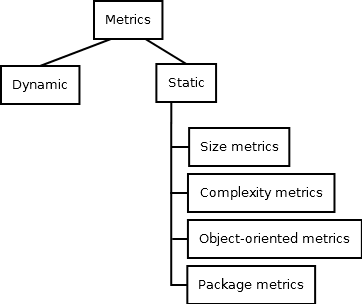
\includegraphics[scale=0.7]{img/Diagram1.png} 
	\caption{Static and dynamic metrics}		
	\label{fig:metrics1}
\end{figure}

The metrics could be also divided into three categories: product metrics, process metrics and project metrics (Figure~\ref{fig:metrics2}). Product metrics describe the characteristics of the product such as size, complexity, design features, performance, and quality level. Process metrics are used to improve maintenance and development of software, for example: the effectiveness of defecting removal during development, the pattern of testing defect arrival, and the response time of the fix process. Project metrics describe the project characteristics and execution, for example: the number of software developers, the life cycle of the software, cost, productivity, and schedule. Metrics could belong to multiple categories. For example, the quality metrics are both process metrics and project metrics \cite{metrics}. 

\begin{figure}[h!]
	\centering
	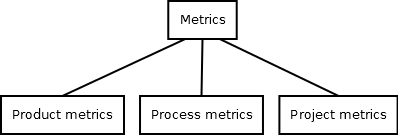
\includegraphics[scale=0.5]{img/Diagram2.png} 
	\caption{Metrics division}		
	\label{fig:metrics2}
\end{figure}


%%%%%%%%%%%%%%%%%%%%%%%%%%%%%%%%%%%%%%%%%%%%%%%%%%%%%%%%%%%%
\section{Software Quality Model}
Experienced software developers are able to create a high quality software, however it is possible only when from the beginning all requirements and expectations are clearly defined. Having the overall view it is possible to design the system that has understandable and minimal complex structure. 

However, the situation often changes after first release. It could happen so, because the client expectations were different or have changed, or new functionality need to be added, or the requirements have been clarified. In that case, the system loses its quality and gets out of control. Testing, maintaining and extending software become a nightmare for developing team. 

In order to keep development projects on the right track, and decrease the consequences of situations described above, several general software quality models gained the acceptance within the software engineering community. First people that described quality models are McCall and Boehm \cite{rigorous}. Figure \ref{fig:boehmjpg} presents Boehm`s view, while Figure \ref{fig:mccalljpg} illustrates how McCall viewed quality.

\begin{figure}[h!]
	\centering
	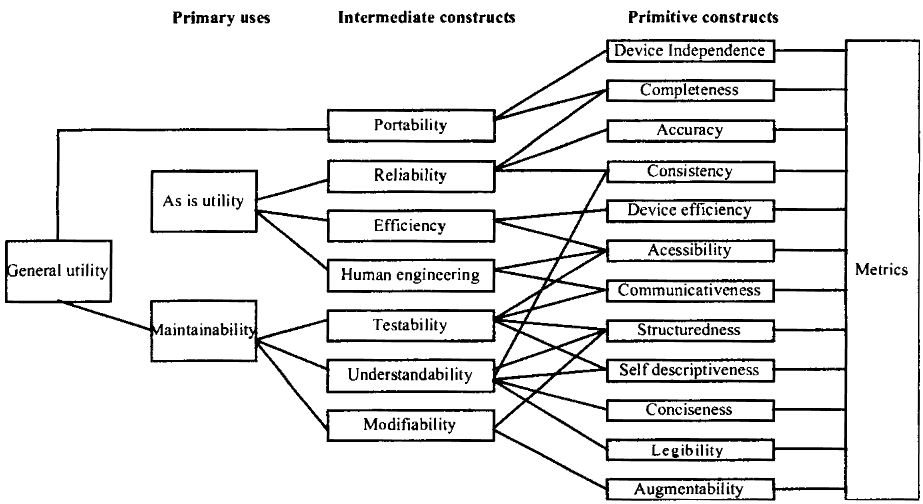
\includegraphics[scale=0.5]{img/boehm-model.jpg}
	\caption{Boehm software quality model (image source:~\cite{rigorous})}		
	\label{fig:boehmjpg}
\end{figure}


\begin{figure}[h!]
	\centering
	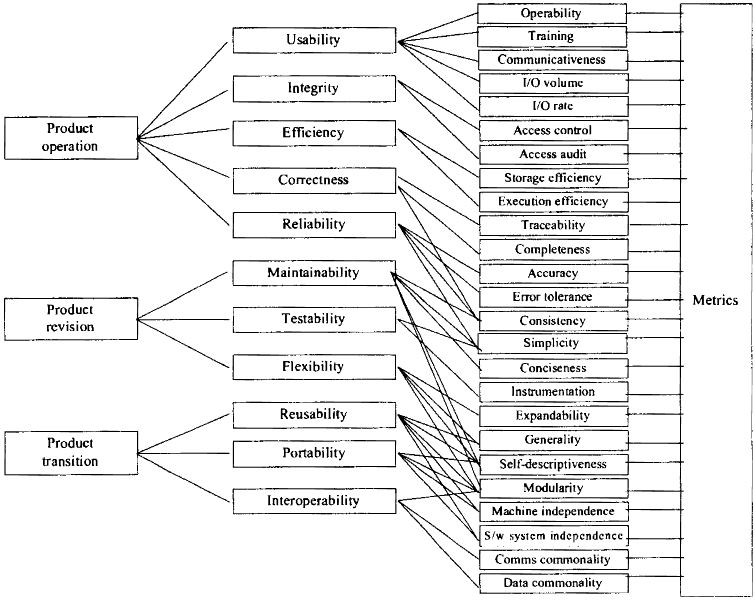
\includegraphics[scale=0.5]{img/mcCall-model.jpg} 
	\caption{McCall software quality model (image source:~\cite{rigorous})}		
	\label{fig:mccalljpg}
\end{figure}

These models focus on the final product (the executable code) and identify the attributes of quality from users point of view. The attributes are called \textit{quality factors}. Because the quality factors names are still too general and no meaningful, they are decomposed into lower-level attributes called \textit{quality criteria}. A further level of decomposition is required when quality criteria are connected to set of low-level, directly measurable attributes called \textit{metrics}. 

\begin{figure}[h!]
	\centering
	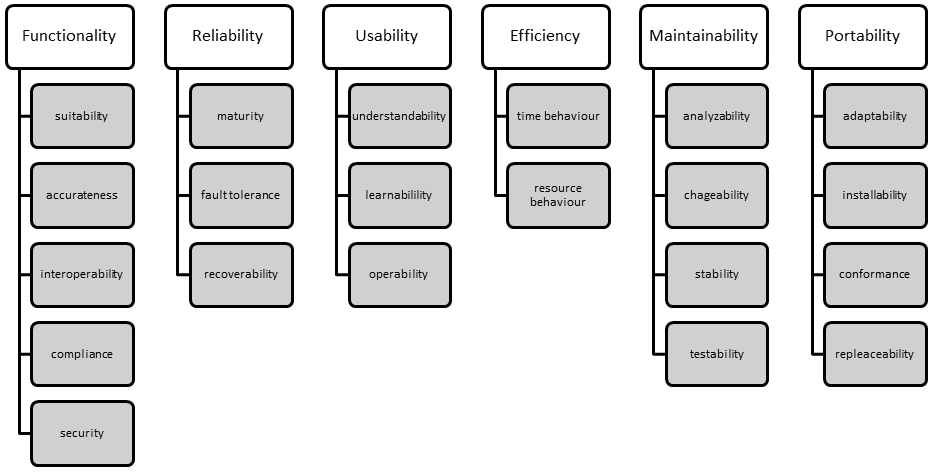
\includegraphics[scale=0.6]{img/diag.png} 
	\caption{The ISO 9126 standard quality model}		
	\label{fig:iso9126}
\end{figure}

From derivation of McCall model, the basic international standard for software quality measurement was defined. The standard is more commonly referenced by its assigned standard number, ISO-9126 (Figure~\ref{fig:iso9126}). It defines software quality as\textit{ ``the totality of features and characteristics of a software product that bear on its ability to satisfy stated or implied needs''} \cite{ISO9126}. The six factors decompose the quality into: 

\begin{itemize}
  \item functionality, 
  \item reliability,
  \item usability,
  \item efficiency,
  \item maintainability,
  \item portability.   
  \end{itemize}
    
\subsection{Functionality}
Functionality is the main purpose of any software. For certain type of software is relatively easy to define its functionality. However, the more functions a software has, the more complicated it becomes. For example, sales order processing systems should be able to record customer information so that it can be used to reference a sales order.

The main point to note is that functionality is expressed as a totality of essential functions that the software product provides. The presence or absence of some functions in a software product can be verified as either existing or not (given function could be or not be found in software product). The other software characteristics present only some degree, because it cannot be simple stated that this characteristic is presented or not. The ISO-9126 quality model does not help measure overall process but only the software component. The relationship between software functionality within an overall business process is outside the scope.

There are five software quality criteria that characterize the usefulness of the software in a given environment (Table~\ref{tab:functionality_factor}):

\begin{table}[h!]
	\centering
\begin{tabular}{|l|l|}
\hline
{\bf quality criteria} & {\bf explanation} \\
\hline
suitability & appropriateness to specification, functions of the software. \\
\hline
accurateness & correctness of the functions \\
\hline
interoperability & ability of software components to interact with other components \\
\hline
compliance & compliant capability of software  \\
\hline
  security & unauthorized access to the software functions \\
\hline
\end{tabular}	
	\caption{\textit{Functionality quality factor}}
	\label{tab:functionality_factor}
\end{table}


\subsection{Reliability}
Reliability is defined as capability of the system to being maintained and its service provision under defined conditions for defined periods of time. From one side of this characteristic is fault tolerance that is the ability of a system to withstand component failure. For example if the connection to the server cannot be established for 30 seconds then system informs the users and follows failure procedures (Table~\ref{tab:reliability_factor}). 

\begin{table}[h!]
	\centering
\begin{tabular}{|l|l|}
\hline
{\bf quality criteria} & {\bf explanation} \\
\hline
  maturity & frequency of failure of the software \\
\hline
fault tolerance & ability of software to withstand (and recover) from failure \\
\hline
recoverability & ability to bring back a failed system to full functionality \\
\hline
\end{tabular}	
	\caption{\textit{Reliability quality factor}}
	\label{tab:reliability_factor}
\end{table}


\subsection{Usability}
Usability is defined with regard to functionality and refers to the ease of use for a given function. For example, the most common functions are exposed on the ribbon to be easily access. The ability to learn how to use a system is also a major sub characteristic of usability. The Table~\ref{tab:usability_factor} depicts the quality criteria of usability.

\begin{table}[h!]
	\centering
\begin{tabular}{|l|l|}
\hline
{\bf quality criteria} & {\bf explanation} \\
\hline
understandability & understanding interaction methods between human and computer \\
\hline
learnability & learning effort for target users \\
\hline
operability & ability of using software in given environment \\
\hline
\end{tabular}	
	\caption{\textit{Usability quality factor}}
	\label{tab:usability_factor}
\end{table}


\subsection{Efficiency}
Efficiency  is concerned with the system resources used to provide required functionality. For example: amount of disk space, memory, network etc. provides a good indication of this characteristic (Table~\ref{tab:efficiency_factor}).

\begin{table}[h!]
	\centering
\begin{tabular}{|l|l|}
\hline
{\bf quality criteria} & {\bf explanation} \\
\hline
time behaviour & response time for user input \\
\hline
resource behavior & refers to hardware resources: cpu, disk, network usage \\
\hline
\end{tabular}	
	\caption{\textit{Efficiency quality factor}}
	\label{tab:efficiency_factor}
\end{table} 


\subsection{Maintainability}
Maintainability is characterized as ability to identify and fix a fault within a software component. It is impacted by code readability or complexity as well as modularization. Quality criteria that help with identification of the cause of a fault and then fixing the fault is the concern of maintainability.  One of the sub characteristics of maintainability is also the ability to verify (or testing) a system (Table~\ref{tab:maintainability_factor}). 

\begin{table}[h!]
	\centering
\begin{tabular}{|l|l|}
\hline
{\bf quality criteria} & {\bf explanation} \\
\hline
analyzability & ability to indentify cause of failure \\
\hline
changeability & amount of effort need to change a system \\
\hline
 stability & impact of system after change  \\
\hline
testability & effort needed to verify a system change \\
\hline
\end{tabular}	
	\caption{\textit{Maintainability quality factor}}
	\label{tab:maintainability_factor}
\end{table}



\subsection{Portability}
Portability is characteristic referring to how well the software could adopt to changes in its environment or with its requirements (Table~\ref{tab:portability_factor}). 

\begin{table}[h!]
	\centering
\begin{tabular}{|l|l|}
\hline
{\bf quality criteria} & {\bf explanation} \\
\hline
adaptability & ability of change after adding extension \\
\hline
installability & effort needed to install software \\
\hline
conformance &  ability to adjust after changing external component (i.e. database) \\
\hline
replaceability & ability to replace any component with other  \\
\hline
\end{tabular}	
	\caption{\textit{Portability quality factor}}
	\label{tab:portability_factor}
\end{table} 

\subsection{Software quality model summary}
Basing on the measurement aspects of quality model, several separate definition could be stated. This definitions reflect the software usage or realities of system testing and, what is more, could be treated as software metrics. 

The simplest example is portability term expressed as:
\begin{equation}
Portability\quad =\quad 1-\frac { ET }{ ER } 
\end{equation} 
where \textit{ET} is a measure of the resources needed to move the system to the target environment and \textit{ER} is a measure of the resource needed to create the system for a resident environment. 

The interpretation of measurements based on quality factors described in ISO-9126, McCall or Boehm models is rather subjective. The objective measurements are more preferable, however the subjective opinion is better than no feedback.  

The comprehensive picture of software quality is presented by six factors. Normally, the measurement should follow  by some defined standards, however, in that case, the methods of measurement and interpretation are defined by end users and developers~\cite{rigorous}.

%%%%%%%%%%%%%%%%%%%%%%%%%%%%%%%%%%%%%%%%%%%%%%%%%%%%%%%%%%%%%%%%%%%%%%%%%%%%%%%%
\section{Size metrics}

Each product of software development could be treated as physical entity and it could be described in terms of its size. It is straightforward and relatively simple to measure. 

\subsection{Lines of Code}
\ac{LoC} is the simplest metric used to measure the size of the program by counting the lines of code. It is the oldest and most widely used size metric. It is very simple concept that have its basics in Assembler programming where every physical line of code was presenting  one instruction. Nowadays, in high level programming languages, the concept have broken down, because of differences between physical lines and instructions statements. As a result, the several variations have been created in order to improve basic \ac{LoC}:

\begin{itemize}
\item \ac{LoC} that counts only executable lines.
\item \ac{LoC} that counts executable lines plus data definitions.
\item \ac{LoC} that counts executable lines, data definitions and comments.
\item \ac{LoC} that counts executable lines, data definitions, comments, and job control language.
\item \ac{LoC} that counts lines as physical lines on a input screen.
\item \ac{LoC} that counts lines as terminated by logical delimiters~\cite{metrics}.
\end{itemize}

There are two major types of  \ac{LoC} measurement: physical \ac{SLoC} and \ac{LLoC}. The specific definition of them are varied. \ac{SLoC} is a line counter in the text of the program's source code including comment and blank lines. \ac{LLoC} attempts to measure number of executable statements, but specific for given computer language. \ac{SLoC} is sensitive to irrelevant code formatting and depends of the programmer code style convention. 

\ac{LLoC} is better metrics, because it estimates the complexity of a single file, class or procedure. Since \ac{LLoC} is not affected by comments, blanks or line continuation, it is a supportive way to measure the amount of the actual programming work. A program with a higher \ac{LLoC} does more than a program with a lower \ac{LLoC}. By adding features, the \ac{LLoC} increases. By deleting features, the \ac{LLoC} should decrease. 

The main advantages of \ac{LoC} is automatic counting,  however used only for a specific language, because it cannot be used for other languages due to the syntax and structural differences among languages.  \ac{LoC} metric is also very intuitive because the effect of it could be visualized. However, there are many disadvantages that underlines the simplicity of this metrics. Using \ac{LoC} it is not possible to measure the productivity of a project. The final number of lines in program is dependent to the experience of the developer,  for instance, the same functionality could be rewritten by experienced developers using smaller number of lines of code. What is more, any form of \ac{LoC} does not take into consideration code redundancy.  There is no standard definition of what a line of code is. It is not clearly defined whether data declarations are included or  does the comments count or  what happens if a statement extends over several lines. 

In relation to \ac{LoC}, several additional terms has been also defined: 
\begin{itemize}
\item KLOC can be used to measure thousands of \ac{LoC}.
\item KDLOC: 1,000 delivered lines of code.
\item KSLOC: 1,000 source lines of code.
\item MLOC: 1,000,000 lines of code.
\item GLOC: 1,000,000,000 lines of code.
\end{itemize}

Summing up, the lines of code metric is one of the oldest and most common forms of software measurement, however is ineffective at comparing the same piece of code of implemented functionality in different languages. It cannot measure the productivity of programmer and code quality~\cite{metrics}.

%%%%%%%%%%%%%%%%%%%%%%%%%%%%%%%%%%%%%%%%%%%%%%%%%%%%%%%%
\subsection{Code coverage}
\label{sec:codecoverage}

Edsger Dijkstra said: \textit{``Testing never proves the absence of faults, it only shows their presence''}.
The code coverage analysis is a measurement used in software testing to describe the degree to which the source code of a program has been tested. There are number of criteria (metrics) that determines how well the tests exercise the code.

The main purpose of code coverage analysis is not only finding the areas of a program not exercised by set of tests, but also creating additional test to increase the coverage or just to identify redundant test cases that does not increase coverage. Using code coverage analysis, it is also important to establish the minimum and maximum percentage of coverage in order to determine when to stop analysing the coverage. 

Code coverage analysis is kind of structural testing technique (other names: glass box testing and white box testing). Structural testing compares behaviour of test program against the direct  intention of the source code. This is a contrast to functional testing (other name: black-box testing) that compares behaviour of test program against a requirements specification. Structural testing examines how the program works, taking into account possible faults in the structure and logic. Functional testing examines what the program accomplishes, without regarding to how it works internally.

There are variety of coverage metrics. The paragraphs below contain a description of some fundamental metrics, their strengths, weaknesses and issues. 

\paragraph{Statement coverage metric} reports every executable statement that is encountered.  Note that a statement does not necessarily correspond to a line of code. Control-flow statements, such as \texttt{if, for} and \texttt{switch} are covered if the expression controlling the flow is covered as well as all the contained statements. Implicit statements, such as an omitted return, are not subject to statement coverage. 

Advantage of statement coverage is verification of what the written code is expected to do and not to do. It also measures the quality of written code, checks the flow of different paths in the program and it also ensures, if those path are tested or not.

Disadvantage of statement coverage is fact that it cannot test the false conditions. It does not report if the loop reaches its termination condition and it does not understand the logical operators.

Statement coverage is also called \textit{statement execution, line, block, basic block} or \textit{segment coverage}.

It could be quite difficult to achieve 100\% statement coverage, because it might be sections of code designed to deal with error conditions, or rarely occurring events. There may also be code that should never be executed.

The statement coverage can be calculated as shown below:
\begin{equation}
Statement\quad coverage\quad =\quad \frac { number\quad of\quad statement\quad exercised }{ total\quad number\quad of\quad statements } \cdot 100\%
\end{equation}


%%%%%%%%%%%%%%%%%%%%%%%%%%%%%%%%%%%%%%%%%%%%%%%%%%%%%%%%
\paragraph{Decision coverage metric} is also known as \textit{branch coverage} or \textit{all-edges coverage}. It covers both the true and false conditions.  A branch is considered as the outcome of a decision and it  simply measures which decision outcomes have been tested. This metrics takes a more in-depth view of the source code than simple statement coverage.

A decision is taken in if-statement, a loop control statement  or a switch statement and the result of these statements could be either TRUE or FALSE.

The advantages of decision coverage is possibility to validate all the branches in the code, because all of them are reached. It is done in order to ensure that no branches lead to any not normal program`s operation. This metric eliminates also problems that occur with statement coverage testing. 

The decision coverage can be calculated as given below:
\begin{equation}
Decision\quad coverage\quad =\quad \frac { Number\quad of\quad decision\quad outcomes\quad exercised }{ Total\quad number\quad of\quad decision\quad outcomes } \cdot 100\%
\end{equation}

The main goal of decision coverage is to ensure if a program could jump and it jumps to all possible destinations. The most simple example is a complete if statement -- listing~\ref{lst:d1}.
\begin{lstlisting}[caption=Decision coverage metric passes,label=lst:d1]
if (x) {
	print "a";
} else {
	print "b";
}
\end{lstlisting}
This coverage is only achieved here only if \texttt{x} is true on one occasion and false on another.

%%%%%%%%%%%%%%%%%%%%%%%%%%%%%%%%%%%%%%%%%%%%%%%%%%%%%%%%
\paragraph{Condition coverage metric} reports the true or false outcome of each condition separately. It measures the conditions independently of each other. It is similar to decision coverage but has better sensitivity to the control flow. During boolean expression evaluation it is need to ensure that all the terms in the expression are exercised -- listing~\ref{lst:d2}.

\begin{lstlisting}[caption=Simple conditional coverage, label=lst:d2]
if (x || y) {
	//...
} 
\end{lstlisting}

In order to achieve the full condition coverage of this expression, the values of \texttt{x} and \texttt{y} are set to each of the four combinations of values they can take:

\begin{verbatim} 
x=true; y=true;
x=true; y=false;
x=false; y=true;
x=false; y=false;
\end{verbatim} 

The condition coverage gets complicated, and difficult to achieve, as the expression gets complicated. For this reason there are a number of different ways of reporting condition coverage which try to ensure that the most important combinations are covered without worrying about less important combinations -- listing~\ref{lst:d3}.

\begin{lstlisting}[caption=Complex conditional coverage, label=lst:d3]
if (a || b) && c {
	//...
}
\end{lstlisting}

The condition will be satisfied by the following set of tests:
\begin{verbatim} 
a=true, b=true, c=true
a=false, b=false, c=false
\end{verbatim} 

However, it does not satisfy the condition coverage, because it need to test rest of possibilities:
\begin{verbatim}
a=false, b=false, c=true
a=true, b=false, c=true
a=false, b=true, c=true
a=false, b=true, c=false
\end{verbatim}

Condition coverage is also known as \textit{expression, condition-decision} and \textit{multiple decision coverage}.
%%%%%%%%%%%%%%%%%%%%%%%%%%%%%%%%%%%%%%%%%%%%%%%%%%%%%
\paragraph{Path coverage metric} reports if every possible path in given function has been followed. This path is a unique sequence of branches from the function entry to the exit. It tests all possible combinations of logical conditions. 

The purpose of path coverage metrics is to ensure that all paths through the program are taken. In sizeable program there will be an enormous number of paths through the program could be executed, so in practice the paths could be limited to those within a single function whether the function is not too big, or i.e. has simply two consecutive branches.

The main advantage of path coverage metrics is accuracy. However, from the other side, the number of paths increase exponentially to the number of branches and it is impossible to exercise all of time in small unit of time.  

%%%%%%%%%%%%%%%%%%%%%%%%%%%%%%%%%%%%%%%%%%%%%%%%%%%%%
\subsubsection{Other coverage metrics} 
There are also many other variation of coverage metrics like\textbf{ function coverage metric} that reports when function or procedure is invoked. The \textbf{call coverage metric} reports every function call. The \textbf{ loop coverage metric} informs whether each loop body has been executed zero times, exactly once or more than once. For supporting multi threading the \textbf{race coverage} reports whether multiple threads execute the same code at the same time. It supports with detecting failures with synchronization of resource access. The \textbf{relational operator coverage} reports if the boundary situations occur with operators: \textit{\textless, \textless=, \textgreater, \textgreater=,==}. 

%%%%%%%%%%%%%%%%%%%%%%%%%%%%%%%%%%%%%%%%%%%%%%%%%%%%%
\subsubsection{Coverage metrics summary}
The result of using statement coverage, decision coverage, or condition coverage should attain 80\%-90\% coverage or more before releasing. It does assure quality and the effort sacrificed to reach this goal, might be supportive in finding more bugs. The good project avoids setting a goal lower than 80\%.

The coverage analysis help eliminate gaps in a test suite. It does not only provide accurate measurements in order to be useful, but also encourage software developers to analyse those results to the minimum detail and support them in decision how code could be improved~\cite{coverage1,coverage2}.

%%%%%%%%%%%%%%%%%%%%%%%%%%%%%%%%%%%%%%%%%%%%%%%%%%%%%
\subsection{Code size metrics summary}
Internal attribute of product like size is important and measuring it directly allows to predict the complexity. Number of characters, lines of code or code coverage is taken into account as a determinant for these kind of metrics.  

Basing on \ac{LoC} it is possible to calculate derivative metrics like productivity quality or \textit{``documentation--size''} metrics: 

\begin{equation}
productivity=\frac { KLOC }{ man-month } 
\end{equation}
 
 \begin{equation}
quality\quad =\quad \frac { bugs }{ KLOC } 
\end{equation}

\begin{equation}
documentation\quad size\quad =\quad \frac{documentation\quad pages }{KLOC} 
\end{equation}

It is worthy to mention that these kind of metrics are only supportive way of monitoring improvement of software development and it is not allowed to evaluate the code developers basing on results of these metrics. 

%%%%%%%%%%%%%%%%%%%%%%%%%%%%%%%%%%%%%%%%%%%%%%%%%%%%%
\section{Complexity metrics}

Computational complexity has also impact on the software, so if the complex algorithms are used in software, there is a need to control the overall efficiency of program execution. The complexity metrics provide the information how complex the implemented methods in code are. The sections below describes the basic and commonly used complexity metrics. 
 
\subsection{McCabe's cyclomatic complexity}
\label{sec:cyclomatic}
McCabe has based its metrics on analysis of some measurement concepts in graph theory. He has  transferred these concepts into domain of software measurement. The terms connected to graph theory have been explained in Chapter~\ref{section:graph_theory} in section: \textit{Graph theory}. The term \textit{cyclomatic number} is explained below (definition from~\cite{alain}).

\begin{quote}
The \textbf{\ac{CC}} number \textit{v(G)} of a strongly connected directed graph is equal to the
maximum number of linearly independent cycles.
\end{quote}\vspace{-1cm}

\begin{equation}
v(G) = e - v + p
\end{equation}

where:
\begin{itemize}\addtolength{\itemsep}{-0.5\baselineskip}\vspace{-7mm}
\item \textit{G} represents the graph,
\item \textit{e} represents the edges of the graph,
\item \textit{v} represents the vertices,
\item \textit{p} represents separate components.
\end{itemize}

The entity being measured is therefore a \textit{``strongly connected directed graph''}. In software, the program is modelled with usage of \textit{control flow graph} that represents abstract structure. In this abstract representation of a program or a procedure, each vertex in the graph represents a basic block, directed edges are used to depicts the jumps in the flow control. There are also two additional designed blocks: entry block through which control flow enters the flow graph and the exit block through which all control flow leaves.  

The Figure~\ref{fig:cyclomatic_complexity} represents the exemplary flow control graph.

\begin{figure}[h!]
	\centering
	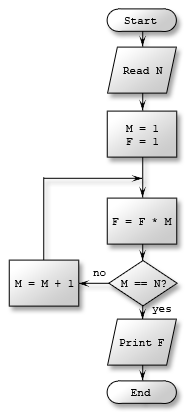
\includegraphics[scale=0.5]{img/cyclomatic_complexity.png} 
	\caption{Example of \ac{CC}: 8 vertices (nodes), 8 edges; $CC = 8 - 8 + 1 = 1$; image source:~\url{http://upload.wikimedia.org/wikipedia/commons/1/16/Flowchart_example.png}.}		
	\label{fig:cyclomatic_complexity}
\end{figure}

In the case of software, the control flow graph is transformed into a strongly connected graph, so graph cyclomatic number could be formulated as:

\begin{equation}
v(G) = e - v + p + 1
\end{equation} 

Furthermore, the individual modules are also taken into consideration, instead of the whole software entity. According to McCabe, the number of connected component $p$ is equal to 1, so the final McCabe equation is formulated as:

\begin{equation}
v(G) = e - v + 2
\end{equation}

where $e$ is a number of edges and $v$ is a number of vertices. It is also another formula that gives the simple \ac{CC} dependent to the number of vertices:

\begin{equation}
v(G) = d + 1
\end{equation}
where $d$ is number of decision vertices points in code where the binary decision are made. This formula allows to quick determination of \ac{CC} value by counting how many in code, the keywords \texttt{if, while, for, switch, case, do, catch} are used. 

The low value of \ac{CC} determines that given function is easy to understand. The greatest value is, the more complicated code is. What is more, the more complex code is, the more faults could appear~\cite{alain}.
%%%%%%%%%%%%%%%%%%%%%%%%%%%%%%%%%%%%%%%%%%%%%%%%%%%%%

\subsection{Halstead complexity}
\label{sec:halstead}

The Halstead's metrics were proposed by Maurice Halstead. The main assumption is to determine a quantitative measure of the complexity directly from the operators and operands in the component. Metrics measure program component's complexity directly from source code, because the implementation or expression of the algorithm should reflect the execution independently of a specific platform. The main goal is to identify measurable software properties and its relations.

Halstead metrics are based on interpretation of the source code as a sequence of tokens and classifying them to be either operator or operand.   

An operand is the part of a computer instruction which specifies what data is to be manipulated or operated on. The operator, in programming, has the same definition as in mathematics. It is a character that represents the specific action performed on the variables (addition, subtraction, multiplication, comparison, incrementation,...). 

The \textbf{program length (\textit{N})} is the sum of the total number of operators and operands in the program:
\begin{equation}
N={ N }_{ 1 }+{ N }_{ 2 }
\end{equation}

The \textbf{vocabulary size (\textit{n})} is the sum of the number of unique operators and operands:
\begin{equation}
n={ n }_{ 1 }+{ n }_{ 2 }
\end{equation}

The \textbf{program volume (\textit{V})} is the contents of program information. It is measured in mathematical bits and is calculated as the program length times the 2-base logarithm of the vocabulary size (\textit{n}) :
\begin{equation}
V=N\cdot \log _{ 2 }{ n } 
\end{equation}

Halstead's volume (\textit{V}) describes the size of the implementation of an algorithm. The computation of \textit{V} is based on the number of operations performed and operands handled in the algorithm. The program volume (\textit{V}) is less sensitive to code layout than the lines-of-code measures\footnote{The definition of Halstead's metrics described above are not a part of complexity metrics, but size metrics, however these metrics are used as a base for metrics describes below which are categorized as complexity metrics. Using Halstead's size metrics is meaningless without Halstead's complexity metrics, so it is a reason why they have been introduced and explained in the same section.}. 

The \textbf{difficulty level or error proneness (\textit{D})} of the program is proportional to the number of unique operators in the program. \textit{D} is also proportional to the ratio between the total number of operands and the number of unique operands. 
\begin{equation}
D=\frac { { n }_{ 1 } }{ 2 } \cdot \frac { { N }_{ 2 } }{ { n }_{ 2 } } 
\end{equation}
        
The \textbf{program level (\textit{L})} is the inverse of the error proneness of the program. I.e. a low level program is more prone to errors than a high level program.
\begin{equation}
L=\frac { 1 }{ D } 
\end{equation}
        
The \textbf{effort to implement (\textit{E})} is proportional to the volume and to the difficulty level of the program. It is also known as program understanding or elementary mental discrimination.
\begin{equation}
E=V\cdot D=\frac { V }{ L } =\frac { { n }_{ 1 }{ N }_{ 2 }{ Nlog_{ 2 }{ n } } }{ 2{ n }_{ 2 } } 
\end{equation}

The \textbf{time to implement (\textit{T})} is proportional to the effort. Empirical experiments could be used for calibrating this quantity. Halstead has found that dividing the effort by Stroud Number $S$ gives an approximation for the time in seconds.
\begin{equation}
T=\frac { E }{ S } =\frac { { n }_{ 1 }{ N }_{ 2 }{ Nlog_{ 2 }{ n } } }{ 2{ n }_{ 2 }S } 
\end{equation}

In 1967, psychologist John M. Stroud suggested that the human mind is capable of making a limited
number of mental discrimination per second (Stroud Number), in the range of 5 to 20. The $S$ value for software scientists is set to 18, thus: 

\begin{equation}
T=\frac { E }{ 18 } 
\end{equation}

\subsection{Complexity metrics summary}
The advantage of Halstead metrics is fact that it does not require in-depth and control flow analysis of program. They are able to predicts an effort and rate the error and estimate the time, so they are useful in scheduling projects. As a drawbacks of Halstead metrics, it could be noticed that it depends on usage of operator and operands in completed code and it has no use in predicting complexity of program at design level.

Calculating the ~\ac{CC} value from the McCabe metric is rather easy. This metric determines also which application elements should be redesigned and reimplemented. However, on the other side, the number of edges in control flow does not give the full answers, because it does not distinguish nested and not nested loops from easy \texttt{case} instruction. It also does not take into account complicated conditions in decision vertices~\cite{complexity1}.


%%%%%%%%%%%%%%%%%%%%%%%%%%%%%%%%%%%%%%%%%%%%%%%%%%%%%%
\section{Object-oriented metrics}
Object-oriented metrics are a response to the object-oriented programming paradigm that is not reflected in the methods of structure programming measurements.   

\subsection{Chidamber \& Kemerer metrics}
\ac{CK metrics} is the set of metrics proposed by S.R.~Chidamber and C.F Kemerer in 1994. They have explored features characteristic for object-oriented design: class complexity, inheritance, coupling and cohesion between classes.   
\paragraph{\ac{WMC}} is a weighted sum of method from given class where single weight is represented as McCabe cyclomatic complexity. \ac{WMC} is a sum of all coefficients of \ac{CC} in given class and is expressed in formula:

\begin{equation}
WMC=\sum _{ i=0 }^{ TM }{ { CC }_{ i } } 
\end{equation}
where $TM$ - number of method in class, $CC_{i}$ - cyclomatic complexity of \textit{i}-method. Recommended \ac{WMC} value should be equal to 20. The value has been determined by NASA scientists. They based its assumptions on experience in object-oriented projects~\cite{nasa}.

\paragraph{\ac{RFC}} is the number of methods that can be invoked in response to a message in a class. In other words, all methods from given class and all methods which are invoked directly by these methods are counted. The greater \ac{RFC} value is, the greater functionality and complexity is. It causes that the cost of testing and maintaining the system also increases. Such value means also more responsible for a class. The desirable value determined by NASA is 40~\cite{nasa}.

\paragraph{\ac{DIT}} is defined as a maximal number of super classes that given class inherits.  The inheritance tree depth are characteristic for complex systems. It involves a wide range of related classes and methods and means higher cost of system maintenance. On the other hand, inheritance increases the reuse of code, which reduces the number of duplicate code~\cite{nasa}.

\paragraph{\ac{NOC}} is defined as sum of all direct class descendants. Large \ac{NOC} values indicate improper usage of inheritance mechanism and might result in difficulties in class testing and maintaining~\cite{nasa}.  

\paragraph{\ac{CBO}} is defined as a number of classes that are coupled with given class using other mechanism than inheritance. The low level of class coupling indicates that class are independent and there are clear boundaries between them. It increases the abstraction of project, because it is easier to modify the code. The high level of \ac{CBO} makes class more sensitive to changes and difficult to maintain, therefore relationship between classes should be kept at as low level as possible. It reduces the complexity of the system and promotes better encapsulation~\cite{nasa}. 

\paragraph{\ac{LCOM}} is type of metric that measures lack of cohesion of methods in class. There are several version of calculating \ac{LCOM}.

\subparagraph*{LCOM1} is a difference between number of pairs of methods that refers to different attributes over the pair of methods referring to at least one common attribute. 

Let the class have $n$ methods $m_{1}, m_{2}, \cdots, m_{n}$ where $I_{j}$ is a set of attributes used by $m_{j}$ method. It could be defined: $P=\left\{ \left( { I }_{ i },{ I }_{ j } \right) :{ I }_{ i }\cap { I }_{ j }=0 \right\}$ and $Q=\left\{ \left( { I }_{ i },{ I }_{ j } \right) :{ I }_{ i }\cap { I }_{ j }\neq 0 \right\}$, so: 

\[LCOM1 = \left\{
  \begin{array}{lr}
    P-Q & if P>Q\\
    0 & otherwise
  \end{array}
\right.
\]

High value indicates that responsibility for given class is too high and class should be divided into smaller, because it is more difficult to test and maintain given class. During next years the \ac{LCOM} metric has been several times redefined. 

\subparagraph*{LCOM2} is represented as per cent of methods that do not have access to individual class attributes. If number of method or attributes is equal to zero, then LCOM2 is also not defined and is equal to zero. 

\begin{equation}
LCOM2=1-\frac { \sum _{ i=1 }^{ TM }{ { Ma }_{ i } }  }{ TM\times TA } 
\end{equation}
where $TM$ is number of method in class, $TA$ is number of attributes in class and $Ma_{i}$ is number of methods that refers to $a_{i}$ attributes. The results of this metric are in interval between 0 and 1. The lowest value, the better is. 

\subparagraph*{LCOM3} is a relative number of methods that do not refer to individual class attributes.

\begin{equation}
LCOM3=\frac { TM-\frac { \sum _{ i=1 }^{ TM }{ { Ma }_{ i } }  }{ TA }  }{ TM-1 } 
\end{equation}

where $TM$ is number of method in class, $TA$ is number of attributes in class and $Ma_{i}$ is number of methods that refers to $a_{i}$ attributes. The results are in interval between 0 and 2. If number of attributes is equal to 0 or number of methods is 1 then metric is not defined. The values greater than 1 indicates lack of cohesion and probability of dividing class on smaller ones in future. 

\subparagraph*{LCOM4} is number of disjoint sets of local methods. Neither of these two sets disjonts. Each two methods within the same set have access to at least one common attributes. Value of this metric is between 0 and $N$ where $N$ is a natural number. Optimal value is equal to 1. For greater values it is need to divide class on smaller classes. 

%%%%%%%%%%%%%%%%%%%%%%%%%%%%%%%%%%%%%%%%%%%%%%%%%%%%%
\subsection{Metrics for Object-Oriented Design (MOOD)}
\ac{MOOD} were created by Fernando Brito e Abreu in 1995. They are expressed in per cents and used to overall system evaluation. It determines the degree of the usage of mechanisms characteristic for object-oriented programming. The \ac{MOOD} set is programming language independent. 

\ac{MOOD} measures the following object-oriented characteristics:

\begin{itemize}\addtolength{\itemsep}{-0.5\baselineskip}\vspace{-7mm}
\item  polymorphism:~\ac{PF};
\item encapsulation (hermatization):~\ac{AHF}~and~\ac{MHF};
\item inheritance:~\ac{AIF}~and~\ac{MIF};
\item messaging:~\ac{CF}.
\end{itemize}\vspace{-10mm}

\paragraph{Polymorphism Factor} defines the degree of classes overridden in subclasses.
\begin{equation}
PF=\frac { \sum _{ i=1 }^{ TC }{ { m }_{ o }({ c }_{ i }) }  }{ \sum _{ i=1 }^{ TC }{ \left[ { m }_{ n }({ c }_{ i })\times dc({ c }_{ i }) \right]  }  } 
\end{equation}
where $TC$ - the number of all classes, $c_{i}$ - the following classes, $m_{n}(c_{i})$ - new methods, $m_{0}(c_{i})$ - inherited methods, $dc(c_{i})$ - descendants of $c_{i}$ class. 

The nominator represents the number of possible different polymorphic situation
and the denominator represents the maximum number of possible distinct polymorphic
situation for class $c_{i}$. Polymorphism enables to link, by its own invocation, many instance of classes, so system becomes more complex and flexible. The typical \ac{PF} value is between 4\% and 18\%. The greater value is, the more complicated inheritance hierarchy is. This situation causes increase the cost of maintenance and testing (\cite{moodbook}, \cite{nasa}). 

\paragraph{Attribute Hiding Factor} defines the degree of attributes encapsulation in class.
\begin{equation}
AHF=\frac { \sum _{ i=1 }^{ TC }{ { a }_{ h }({ c }_{ i }) }  }{ \sum _{ i=1 }^{ TC }{ { a }_{ d }({ c }_{ i }) }  }
\end{equation}
where $TC$ - the number of all classes, $c_{i}$ - the following classes, $a_{h}$ - non-public attributes, $a_{d}$ - all defined attributes in $c_{i}$ class. The~\ac{AHF} value should be close to 100\% because it is one of basic assumption of encapsulation that attributes are only accessible using methods~\cite{moodbook, nasa}.

\paragraph{Method Hiding Factor} defines the degree of method encapsulation in class.
\begin{equation}
MHF=\frac { \sum _{ i=1 }^{ TC }{ { m }_{ h }({ c }_{ i }) }  }{ \sum _{ i=1 }^{ TC }{ { m }_{ d }({ c }_{ i }) }  } 
\end{equation}
where $TC$ - the number of all classes, $c_{i}$ - the following classes, $m_{h}$ - non-public methods, $m_{d}$ - all defined methods in $c_{i}$ class. The desirable value of~\ac{MHF} should be between 10\% and 25\%, because some of methods are not available at all~\cite{moodbook, nasa}.


\paragraph{Attribute Inheritance Factor} defines the degree of attributes inheritance usage. It is a ratio of inherited and all available attributes. 
\begin{equation}
AIF=\frac { \sum _{ i=1 }^{ TC }{ { a }_{ i }({ c }_{ i }) }  }{ \sum _{ i=1 }^{ TC }{ { a }_{ a }({ c }_{ a }) }  } 
\end{equation}
where $TC$ - number of all classes, $a_{a}(c_{i}) = a_{d}(c_{i}) + a{i}(c{i})$ - public attributes in $c_{i}$ class, $a_{i}(c_{i})$ - inherited and not overridden attributes in $c_{i}$ class, $a_{d}(c_{i}) = a_{n}(c_{i}) + a_{o}(c_{i})$ - attributes defined in $c_{i}$ class, where $a_{n}(c_{i})$ - new attributes, $a_{o}(c_{i})$  - inherited and overridden attributes. The typical value of \ac{AIF} is between 50\% and 60\%~\cite{moodbook, nasa}.  


\paragraph{Method Inheritance Factor} defines the degree of methods inheritance usage. It is a ratio of inherited and all available methods. 
\begin{equation}
MIF=\frac { \sum _{ i=1 }^{ TC }{ { m }_{ i }({ c }_{ i }) }  }{ \sum _{ i=1 }^{ TC }{ { m }_{ a }({ c }_{ a }) }  } 
\end{equation}
where $TC$ - number of all classes, $m_{a}(c_{i}) = m_{d}(c_{i}) + m_{i}(c_{i})$ - public methods in $c_{i}$ class, $m_{i}(c_{i})$ - inherited and not overridden methods in $c_{i}$ class, $m_{d}(c_{i}) = m_{n}(c_{i}) + m_{o}(c_{i})$ - methods defined in $c_{i}$ class, where $m_{n}(c_{i})$ - new methods, $m_{o}(c_{i})$  - inherited and overridden methods. The typical \ac{MIF} value is between 65\% and 80\%. The values below indicates weak usage of inheritance, otherwise, the values greater than 80\% complicates the inheritance and code re-usage~\cite{moodbook, nasa}. 


\paragraph{Coupling Factor} defines the degree of coupling between classes using different methods than inheritance. It is a ratio of number of couplings between classes with use of aggregation, composition, association and maximal number of couplings that could be used in system.  
\begin{equation}
CF=\frac { \sum _{ i=1 }^{ TC }{ \left[ \sum _{ j=1 }^{ TC }{ is\_ client\left( { c }_{ i },{ c }_{ j } \right)  }  \right]  }  }{ { TC }^{ 2 }-TC+2\times \sum _{ i=1 }^{ TC }{ dc({ c }_{ i }) }  } 
\end{equation}	
where $TC$ - number of all classes, $dc(c_{i})$ - descendants of $c_{i}$ class, ${TC}^{2}-TC$ - maximal number of possible couplings in $TC$ class system, $2\times \sum _{ i=1 }^{ TC }{ dc({ c }_{ i }) }$ - maximal number of coupling using inheritance in system,  $is\_ client\left( { c }_{ i },{ c }_{ j } \right) = 1\quad if\quad { c }_{ c }\Rightarrow { c }_{ s }\wedge { c }_{ c }\neq { c }_{ s }\wedge \neg \left( { c }_{ c }{ \rightarrow c }_{ s } \right) $ otherwise $is\_ client\left( { c }_{ i },{ c }_{ j } \right) =0$. The ${ c }_{ c }\Rightarrow { c }_{ s }$ expression means that class $c_{c}$ has at least one reference to class $c_{s}$. The ${ c }_{ c }{ \rightarrow c }_{ s }$ expression means that  class $c_{c}$ inherits class $c_{s}$. The \ac{CF} value is between 5\% and 15\%. The high value means that system is not flexible and is difficult to maintain and test, because one change in the system requires modifications in another parts of system. Small value means that classes are too complex, not cohered and it realizes too much functionality inside~\cite{moodbook, nasa}.
	%%%%%%%%%%%%%%%%%%%%%%%%%%%%%%%%%%%%%%%%%%%%%%%%%%%%%%
\section{Package metrics}

Package metrics are used to measure software at the package level. They are used to evaluate the correctness of coupling. The most popular set of package metrics were introduced by Robert C. Martin.

\subsection{Martin metrics}
Martin metrics are set of five metrics designed by Robert Cecil Martin in 1994. His metrics \textit{``can be used to measure the quality of an object-oriented design in terms of the interdependence between the subsystems of that design, because designs which are highly interdependent tend to be rigid, unreusable and hard to maintain''}~\cite{martin}.

\paragraph{\ac{Ce}} is also known as \textit{Outgoing Dependencies}. This metric measures all the types from the source of the measured package referring to the types not in the measured package~\cite{martin}. A large \ac{Ce} indicates that a package is unfocussed and unstable, because it depends on the stability of all the types to which it is coupled. The recommended value of \ac{Ce} is upper limit of 20. The \ac{Ce} could be reduced by extracting some parts of classes and decomposing into smaller and more specialized classes. The typical example of large valued efferent coupling are GUI elements which covers all logical operation within a software.

\paragraph{\ac{Ca}} determines how many classes and interfaces from other packages depend on classes in analysed package. It is also known as \textit{Incoming Dependencies}. The number of packages that depend on the analysed package indicates the package level of responsibility. If the package is relatively abstract then a large number of incoming dependencies is acceptable. Otherwise if not, the package is more concrete. The acceptable values are much larger than in the case of \ac{Ce}. The allowed value for \ac{Ca} is about 500. It is caused by difficulty of the control of the packages which depend on the analysed package. An example of \ac{Ca} high value is controller from MVC pattern~\cite{martin}.

\paragraph{\ac{I}} is measured by calculating the effort necessary  to change a package without impacting other packages within the application. Instability is also called \textit{Stable Dependencies Principle}. The number of incoming and outgoing dependencies is an indicator that determines the stability and instability of a package. Instability can be calculated by comparing the incoming and outgoing package dependencies:

\begin{equation}
I\quad =\quad \frac { Ce }{ Ca+Ce } 
\end{equation}

The returned value is in the range between 0.0 and 1.0 where 0.0 indicates a maximally stable package and 1.0 indicates a maximally unstable package. However, it is impossible to clearly state about stability of package, so it have been assumed that package is stable within range: 0.0 to 0.3 and unstable from 0.7 to 1.0.

Summing up, the package containing multiple outgoing but few incoming dependencies is less stable because of the consequences after introducing changes. On the other hand, package containing more incoming dependencies are more stable because it is more difficult to change~\cite{martin}.


\paragraph{\ac{A}} calculate a relationship between number of  abstract classes and interfaces within package and total number of concrete (non-abstract) classes in the same package. The abstractness is calculated using the formula:

\begin{equation}
A=\frac {N_{a}}{N_{c}} 
\end{equation}

where $N_{a}$ is a number of abstract classes and interfaces in a package and $N_{c}$ is a number of concrete classes and interfaces in the package. The abstractness value of zero ($A=0$) indicates that package contains complete concrete classes. The abstractness value of one ($A=1$) indicates that package is completely abstract. 

Having abstractness value in range between 0 and 0.5 determines that package is opened to changes of implementation. However it could be stated so, whether this value will be compared to instability of package. If package is highly unstable, it would be hard to change because of stability and such package cannot be extended because it is not abstract.

If the abstractness value is closed to 1, the package is unstable and it should consist of concrete classes. It is need to limit dependences to unstable types. Using abstract classes as unstable types will cause increased of dependences to them, because, in case of abstract classes, it is need to create class that will inherit from abstract class~\cite{martin}.


\paragraph{\ac{D}} points that abstractness and stability of packages are closely connected. This metrics is expressed using the formula:

\begin{equation}
D = A + I - 1
\end{equation}

The ideal value is $D=0$, what means that the more abstract a package is, the more stable it should be because it should have many clients that depend on its abstractions. The desirable value should as low as possible~\cite{martin}. Any package that is not closed to zero is considered as unbalanced and should be reimplemented in order to be more reusable and less sensitive to changes.

\section{Other software metrics}
\label{sec:other-metrics}
There are also many other software metrics that are commonly used to preventing the faults in software. They increase the quality of code and have been implemented in plugins in Eclipse IDE described in Chapter~\ref{roz:metrics-tools}. The alphabetic list presents short description of each of them:  

\textbf{\ac{CLOC}} counts all lines that contain regular comments and Javadoc comments.

\textbf{\ac{COM}} calculates number of comment lines. 

\textbf{\ac{CYC}} estimates how many cycles in which a package is involved.

\textbf{\ac{DC}} determines a density value of how commented the code is and is expressed in formula: $DC = \frac{CLOC}{LOC}$.

\textbf{\ac{DIP}}  calculates the ratio of dependencies that have abstract classes or interfaces as a target.

\textbf{\ac{DCYC}} counts every mutual dependency between packages.

\textbf{\ac{EP}}  calculates the ratio of classes that are used outside of a package.

\textbf{\ac{EXEC}} counts the number of executable statements.	

\textbf{\ac{LC}} indicates density of comments with respect to textual size of program $LC=\frac {LOC}{COM}$.

\textbf{\ac{LSP}} is the number of direct subpackages of a package.

\textbf{\ac{NOA}}  calculates the number of fields declared in class or interface.

\textbf{\ac{NCLOC}} (aka NCSL and ELOC) counts all the lines that do not contain comments or blank lines.

\textbf{\ac{NOF}}  calculates the number of fields declared in method.

\textbf{\ac{NOM}} indicates number of modules (packages).

\textbf{\ac{NOTa}} counts the number of abstract classes and interfaces.

\textbf{\ac{NOTc}} counts the number of concrete classes.	

\textbf{\ac{NOTe}} counts the number of classes and interfaces exported outside a package.

\textbf{\ac{NP}} counts the number of parameters for a method or a constructor.

\textbf{\ac{NOT}} counts the number of classes and interfaces.

\textbf{\ac{MC}} indicates density of comments with respect to logical complexity of program $LC=\frac { CC }{ COM } $.

\section{Summary}
The described metrics supports the software developers to keep their projects on the right track. The quality of the provided final product is more resistant on faults and it often does not require releasing additional patches in future. Metrics are particularly useful when the software is further developed and there is no chance to redefine or rebuild some components of the system.

The main advantage of software metrics is fact that they are able to verify the laws and rules of structural and object-oriented programming. In other words, they teach and support the good coding practise that is very important issue when the complex system is implemented and developed.

The aspects of programming and software developing that are measured by presented software metrics does not fully determines the quality of final software product. The difference between languages fundamentals and syntax does require to define or redefine some definitions again. For example, the \ac{DIT} and \ac{NOC} metrics from \ac{CK metrics} does not take into consideration the multi-inheritance.   

Metrics could be treated as useful tool for code understanding, however most of the scientific publications about metrics comes from nineties. It proves that the issue is not interesting matter of study now. What is more, it is still many open cases and new metrics could be defined or existing ones become specific and more detailed.
                
%practical
\chapter{Tools implementing software metrics} \label{roz:metrics-tools}

This chapter describes the tools (part of them are plug-ins for Eclipse IDE) that implements software metrics. Part of them are command-line applications. There are presented not only professional tools provided by software companies, but also created by academic teams and individual developers. The final conclusions and indication of the best tools are in the summary of the chapter. The tools are presented in alphabetical order.
%%%%%%%%%%%%%%%%%%%%%%%%%%%%%%%%%%%%%%%%%%%%%%%%%%

\section{C and C++ Code Counter}
C and C++ Code Counter (CCCC) is a command line tool developed by Tim Littlefair. It is freeware and open source interface designed for Linux and Windows platform. Firstly, CCCC were implemented to process C-family language files (C++ and ANSI C), however last versions are able to process Java source files as well. The installation and running process on the command line is rather easy. CCCC checks the extension of name of file, and if the extension is known and indicates a supported language, the appropriate parser runs file analysis. Final output of the analysis is generated in HTML and XML files. Despite the fact, that HTML summary is not eye-catching, it is a readable and clear summary of analysis made by CCCC tool (Figures~\ref{fig:cccc1} and \ref{fig:cccc2}). While the XML version is rather difficult to read, analyse and understand (Listing~\ref{ccccXml}). 

\begin{figure}[h!]
	\centering
	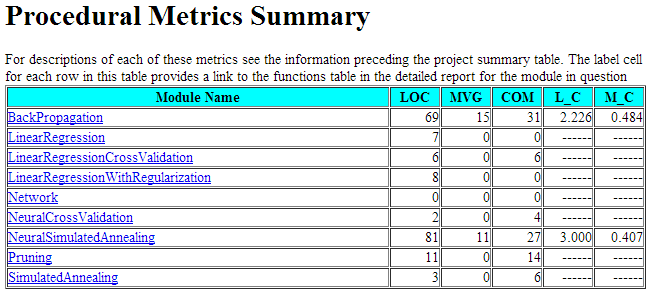
\includegraphics[scale=0.6]{img/cccc1.png} 
	\caption{Procedural metrics summary generated by CCCC metric tool (\ac{NOM}, \ac{COM}, \ac{LC}, \ac{MC})}		
	\label{fig:cccc1}
\end{figure}

\begin{figure}[h!]
	\centering
	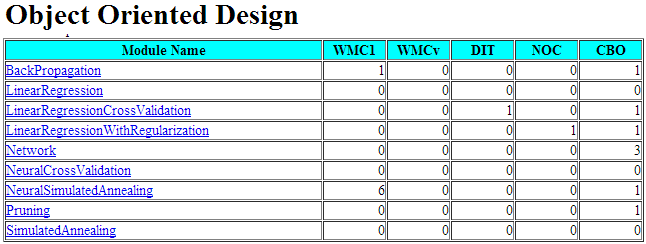
\includegraphics[scale=0.6]{img/cccc2.png} 
	\caption{Object Oriented Design summary generated by CCCC metric tool}		
	\label{fig:cccc2}
\end{figure}

CCCC produces various measures such as size metrics, complexity metrics, object oriented metrics defined by Chidamber and Kemerer~\cite{indie, vaxjo, cccc1}.

CCCC could be downloaded from \textit{sourceforge.net} servers\footnote{CCCC download - \url{http://sourceforge.net/projects/cccc/} (access: November 25, 2013).} and detailed user guide is available on Tim Littlefair official page\footnote{CCCC user guide - \url{http://www.stderr.org/doc/cccc/CCCC\%20User\%20Guide.html} (access: November 25, 2013).}.

\begin{lstlisting}[caption=XML representation of results generated by CCCC metric tool, label=ccccXml]
<?xml version="1.0" encoding="utf-8"?>
<!--Detailed report on module Network-->
<CCCC_Project>
<module_summary>
<lines_of_code value="0" level="0" />
<lines_of_code_per_member_function value="******" level="0" />
<McCabes_cyclomatic_complexity value="0" level="0" />
<McCabes_cyclomatic_complexity_per_member_function value="******" level="0" />
<lines_of_code value="0" level="0" />
<lines_of_code_per_member_function value="********" level="0" />
<lines_of_code_per_line_of_comment value="------" level="0" />
<McCabes_cyclomatic_complexity_per_line_of_comment value="------" level="0" />
<weighted_methods_per_class_unity value="0" level="0" />
<weighted_methods_per_class_visibility value="0" level="0" />
<depth_of_inheritance_tree value="0" level="0" />
<number_of_children value="0" level="0" />
<coupling_between_objects value="3" level="0" />
...
</CCCC_Project>
\end{lstlisting}

%%%%%%%%%%%%%%%%%%%%%%%%%%%%%%%%%%%%%%%%%%%%%%%%%%%%%%%%%%%
\section{Chidamber and Kemerer Metrics}
Chidamber and Kemerer Metrics (CKJM) is an open source command-line tool which calculates object-oriented metrics proposed by Chidamber and Kemerer. This tool processes the byte-code of compiled Java files. 

To run \textit{CKJM} the following line need to be executed\footnote{\textit{CKJM} tool could be download from: \url{http://www.spinellis.gr/sw/ckjm/doc/indexw.html} (access: November 25, 2013).}:

\begin{verbatim} 
java -jar [localization of ckjm.jar] [localization of *.class files] 
\end{verbatim} 

The command's output will be a list of class names (prefixed by the package they are defined in), followed by the corresponding metrics for that class: \ac{WMC}, \ac{DIT}, \ac{NOC}, \ac{CBO}, \ac{RFC}, \ac{LCOM}, \ac{Ce}, and NPM - number of public methods for a class (last two are not \ac{CK metrics}). The exemplary output is presented below:

\begin{verbatim} 
Algorithms.NeuralSimulatedAnnealing 6 1 0 3 28 0 0 3 2 0,7667 328 0,8333 
0 0,0000 0,3333 0 0 52,6667
 ~ private void changeWeights(): 4
 ~ private double[] changeWeightsArray(double[] weights): 2
 ~ private void feedforward(): 2
 ~ public void annealNetwork(): 4
 ~ public void <init>(NeuronNetworkLibrary.Network network, long cycles, 
 double startingTemp, double stopTemp): 1
 ~ private void revertWeights(): 4
\end{verbatim} 

The form of results presentation is definitely not intelligible and comparing to other tools is rather out-of-date.  


%%%%%%%%%%%%%%%%%%%%%%%%%%%%%%%%%%%%%%%%%%%%%%%%%%
\section{Cobertura}
Cobertura\footnote{Cobertura official page - \url{http://cobertura.github.io/cobertura/} (access: November 25, 2013).} is a freeware tool that checks code coverage metrics, but it also implements Cyclomatic Complexity.  It uses compiled Java class files and generates output report in XML or HMTL format. Reports shows percentage test coverage on different levels like packages, classes and methods (Figure~\ref{fig:coverage1}). 

\begin{figure}[h!]
	\centering
	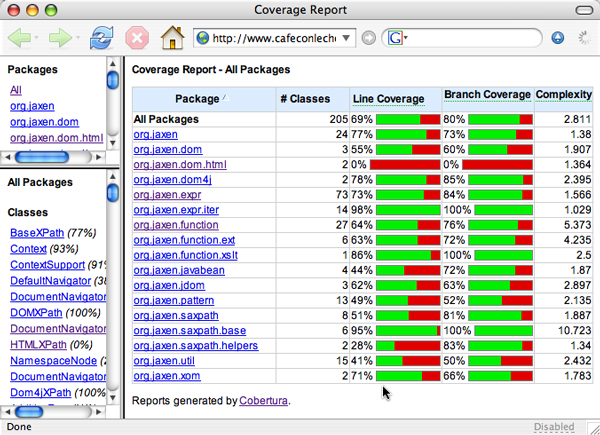
\includegraphics[scale=0.5]{img/coverage.jpg} 
	\caption{HTML report generated by Cobertura (image source: \url{http://tnijurl.com/58c65644bde2/}, access: November 25, 2013)}		
	\label{fig:coverage1}
\end{figure}

Cobertura is run with use of command line or Ant task. It is distributed also as a plugin for Eclipse IDE and is named eCobertura (Figure~\ref{fig:coverage2}). 

\begin{figure}[h!]
	\centering
	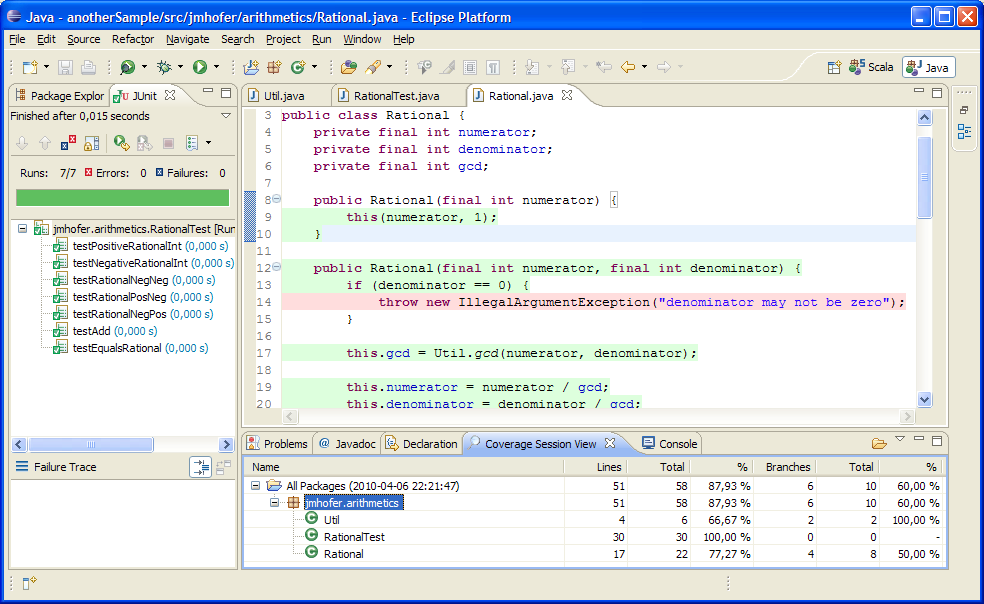
\includegraphics[scale=0.4]{img/screenshot_ecobertura_01.png}  
	\caption{eCobertura as a plug-in for Eclipse IDE (image source: \url{http://ecobertura.johoop.de/},  access: November 25, 2013)}		
	\label{fig:coverage2}
\end{figure}


%%%%%%%%%%%%%%%%%%%%%%%%%%%%%%%%%%%%%%%%%%%%%%%%%%%%%%%%%%%
\section{Eclipse Metrics Plug-in 1.3.6}
Eclipse Metrics Plug-in is an open source metrics calculator plug-in for the Eclipse IDE. It detects
cycles in package, dependencies types and measures various metrics like size metrics (\ac{LoC}, number of classes, number of children, number of interfaces), Martin's metrics and \ac{CK metrics}. 

The plug-in is available to download from \textit{sourceforge.net} servers\footnote{Eclipse Metrics Plug-in 1.3.6 - \url{http://metrics.sourceforge.net/}  (access: November 25, 2013).}. In Eclipse, the result of measurement are presented in \textit{Metrics View} where red colour shows which metrics values exceed assumed values and blue one shows which values are accepted (Figure~\ref{fig:eclipsemetrics}). The whole interface is configurable and is handy tool for developers during implementation. 

The results of metrics could be exported to XML file. The scope of the report (project, package, etc.) is selected from context menu.

\begin{figure}[h!]
	\centering
	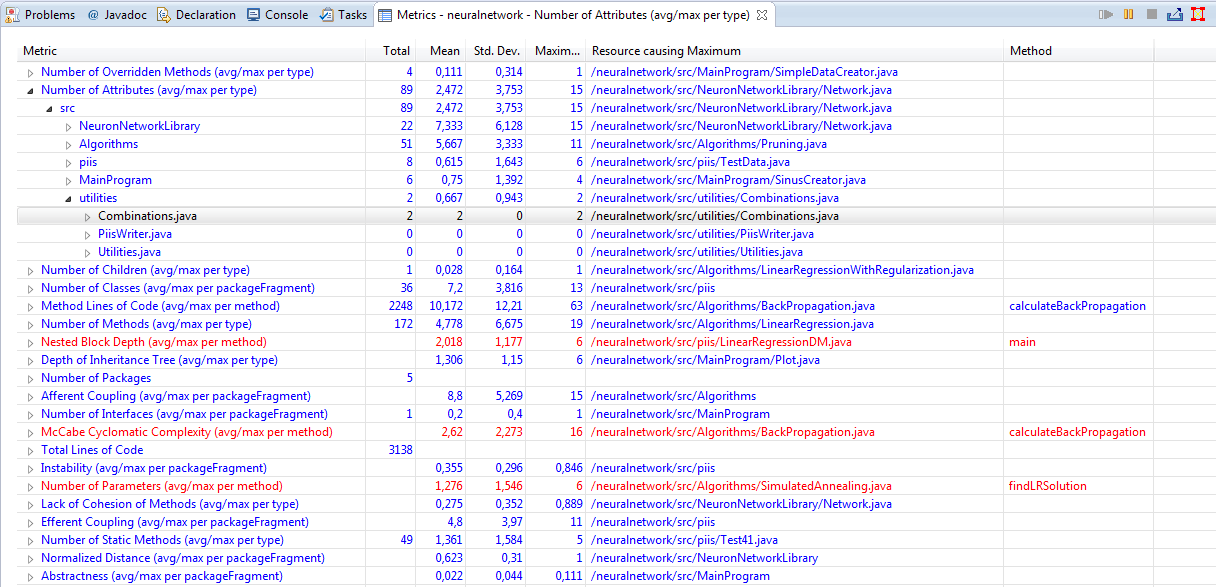
\includegraphics[scale=0.45]{img/eclipse-plugin.png} 
	\caption{Eclipse Metrics Plug-in}		
	\label{fig:eclipsemetrics}
\end{figure}


%%%%%%%%%%%%%%%%%%%%%%%%%%%%%%%%%%%%%%%%%%%%%%%%%%%%
\section{JHawk}
JHawk is shareware metric tool for Java language. It is distributed as stand-alone GUI application or a command line application or as an Eclipse plug-in. The results of measurement is provided in commonly used formats: CSV, XML and HTML. Demo version of JHawk could be downloaded from official website\footnote{JHawk official page - \url{http://www.virtualmachinery.com/jhawkprod.htm} (access: November 25, 2013).}.

JHawk is advanced measurement tool. The GUI or plugin version provides a dashboard tab which gives overview of the metrics at System, Package and Class level, so the interface is really intuitive and user-friendly. The data are presented in readable and intelligible way. What is more, this tool enables also to create own metrics (Figures~\ref{fig:jhawk1}~and~\ref{fig:jhawk2}).

JHawk implements size metrics: Lines of Code, Lines of Comments, Lines of Statements and Expressions; complexity metric created by Halstead (Halstead metrics) and object-oriented metrics created by Chidamber and Kemerer. 

\begin{figure}[h!]
	\centering
	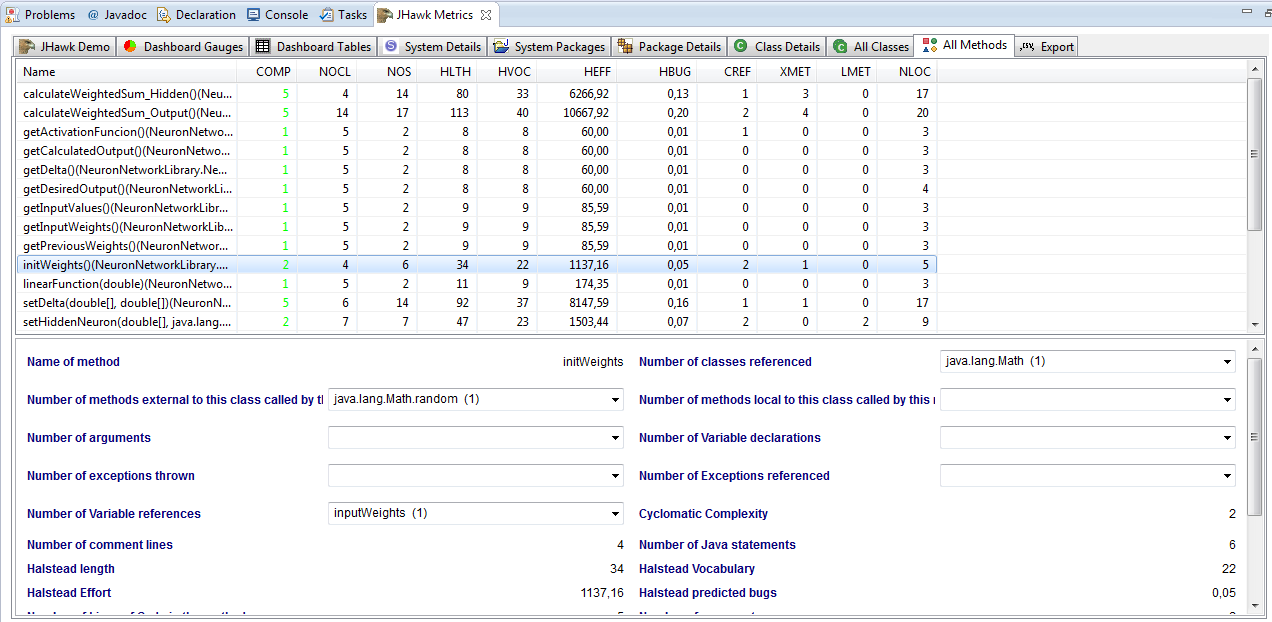
\includegraphics[scale=0.45]{img/jhawk1.png} 
	\caption{JHawk: All Methods View}		
	\label{fig:jhawk1}
\end{figure}

\begin{figure}[h!]
	\centering
	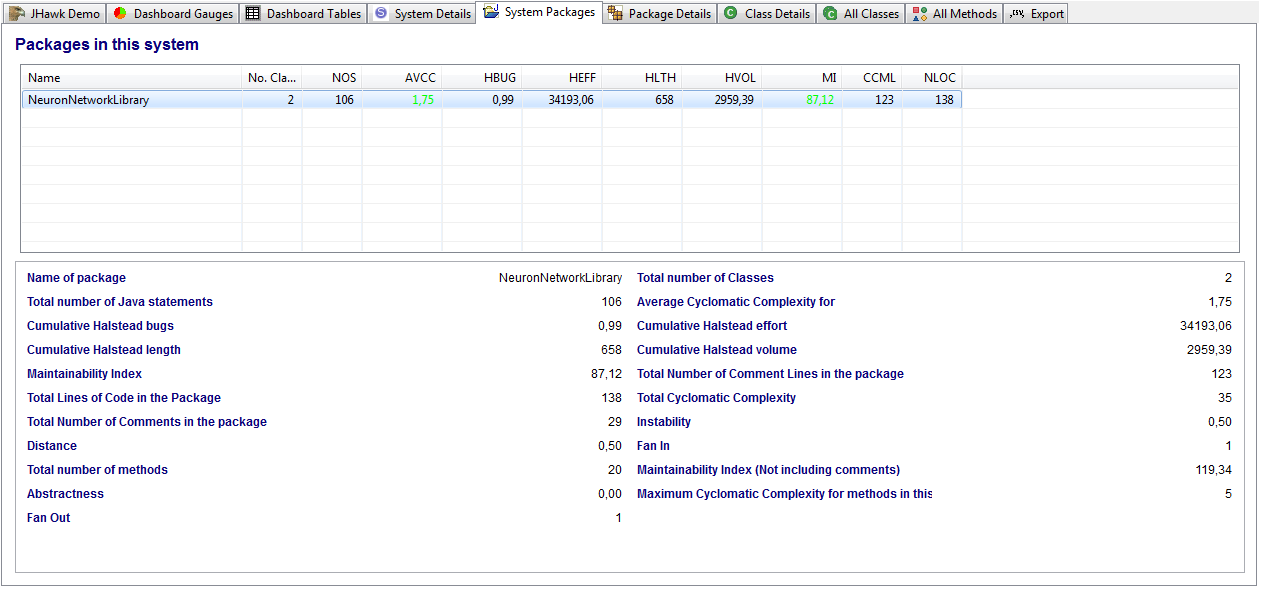
\includegraphics[scale=0.45]{img/jhawk2.png}  
	\caption{JHawk: System Packages View}		
	\label{fig:jhawk2}
\end{figure}

%%%%%%%%%%%%%%%%%%%%%%%%%%%%%%%%%%%%%%%%%%%%%%%
\section{RefactorIT}
RefactorIT provides not only source-code metrics, but also supports automated refactoring process, audits and corrective actions. It is installed as a stand-alone application or as a plug-in to Eclipse or NetBeans. It was commercial tool developed by Aqris company. Since 2008, the RefactorIT is an abandoned project and is freely accessed.  

The plug-in is still available to download on \textit{sourceforge.net} servers\footnote{RefactorIT official page - \url{http://refactorit.sourceforge.net/} (access: November 25, 2013).}. The detailed user guide has been prepared by the student of Pennsylvania University\footnote{RefactorIT user guide - \url{http://tnijurl.com/0472430909e9/} (access: November 25, 2013).}.  

RefactorIT implements large set of metrics:
\begin{itemize}
\item size metrics: \ac{LoC}, \ac{CLOC}, \ac{DC}, \ac{EXEC}, \ac{NOT}, \ac{NOTa}, \ac{NOTc}, \ac{NP}, \ac{NOF}, \ac{NOA} (description of these metrics in section~\ref{sec:other-metrics});
\item complexity metric:~\ac{CC};
\item Martin's metrics;
\item \ac{CK metrics} without \ac{LCOM} and \ac{CBO}.
\end{itemize}
 
RefactorIT generates a report in text, HTML and XML format with values from all selected metrics analyse for all types of level. It gives the possibility of further analysis of metrics based on all the values collected from the entire project or selected package, component or module. 
 
In Eclipse IDE, the values of metrics that  exceeded admissible values are marked on red (Figure~\ref{fig:refactor2}). The exceeded values are also changeable and could be set before starting process of metrics measurement (Figure~\ref{fig:refactor1}). 
 
\begin{figure}[h!]
 	\centering
 	 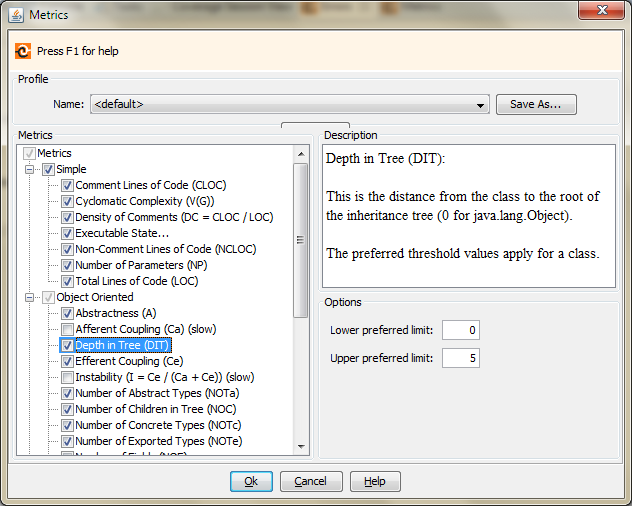
\includegraphics[scale=0.6]{img/refactorit1.png} 
 	\caption{RefactorIT: choice of metrics used to prepare a final measurement report, there is also a short description of each metrics}		
 	\label{fig:refactor1}
 \end{figure} 

\begin{figure}[h!]
	\centering
	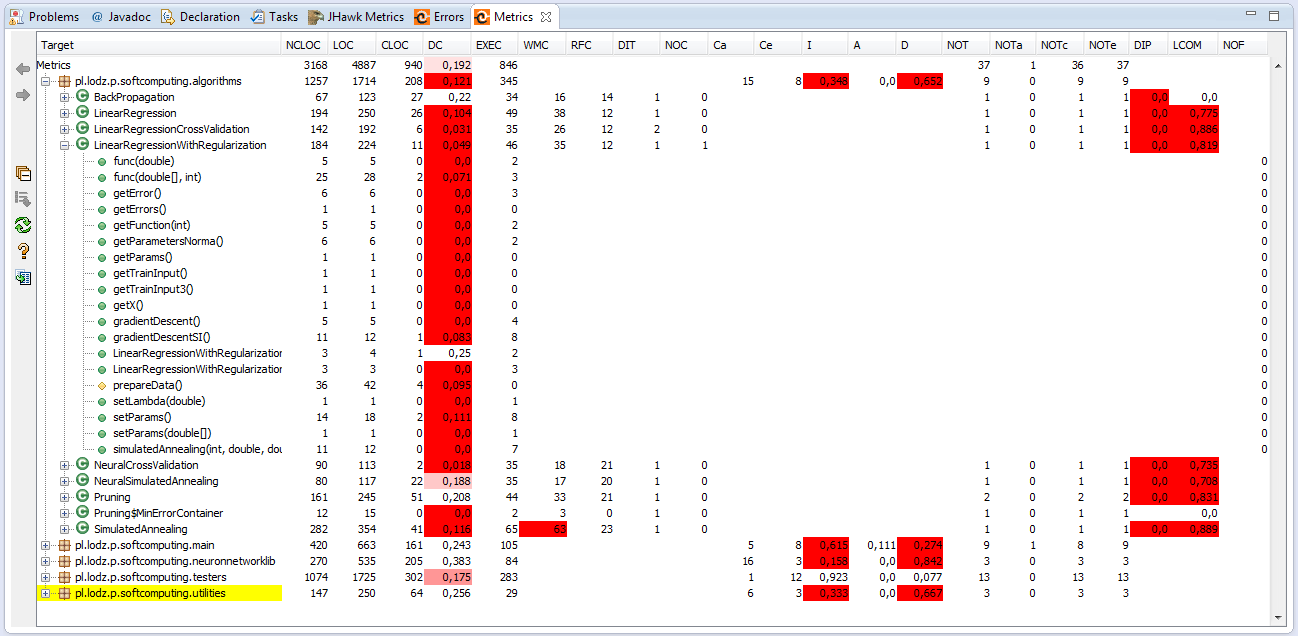
\includegraphics[scale=0.45]{img/refactorit2.png}  
	\caption{RefactorIT: the results of metrics measurement in Eclipse IDE}		
	\label{fig:refactor2}
\end{figure}

%%%%%%%%%%%%%%%%%%%%%%%%%%%%%%%%%%%%%%%%%%%%%%%%%
\section{SonarQube}
SonarQube (previously known as \textit{``Sonar''}) is open-source platform used to maintain a quality of software. Originally, it was designed to analyse software written in Java, but set of additional plug-ins extends possibility to support: Android, C, C++, Cobol, C Sharp, Flex, JavaScript, PHP, PL/SQL and Visual Basic. Nowadays, it is the fastest developing platform that supports code metrics. It is used by many software companies and programmer teams. It is fully integrated with Maven, Ant, continuous integration tools (Atlassian Bamboo, Jenkins), IDEs (Eclipse) and bug tracking systems (JIRA).    

The installation files are ready to download from official page of SonarQube\footnote{SonarQube official page - \url{http://www.sonarqube.org} (access: November 25, 2013).}. It is also required to install server environment (Tomcat) and database. 

The set of metrics supported in SonarQube is also very rich:

\begin{itemize}
\item size metrics:  \ac{LoC}, \ac{COM}, \ac{DC}, \ac{NOM}, \ac{EXEC}, number of classes,  number of methods, number of getters and setters methods and code coverage (description of some of these metrics in sections~\ref{sec:other-metrics} and~\ref{sec:codecoverage});
\item complexity metric:~\ac{CC};
\item \ac{CK metrics};
\item Martin's metrics: \ac{Ca} and \ac{Ce} metric.
\end{itemize}

The main advantages of SonarQube are efficient way of navigating and elaborated balance in high-level view of dashboard supporting in faults detection (Figure~\ref{fig:sonar1}). What is more, it is a web-based application, so the overall rules, alerts, exclusions, settings are configurable in web browser. It not only allows to combine metrics altogether, but also to mix them with chronological measures (Figure~\ref{fig:sonar2}).

\begin{figure}[h!]
	\centering
	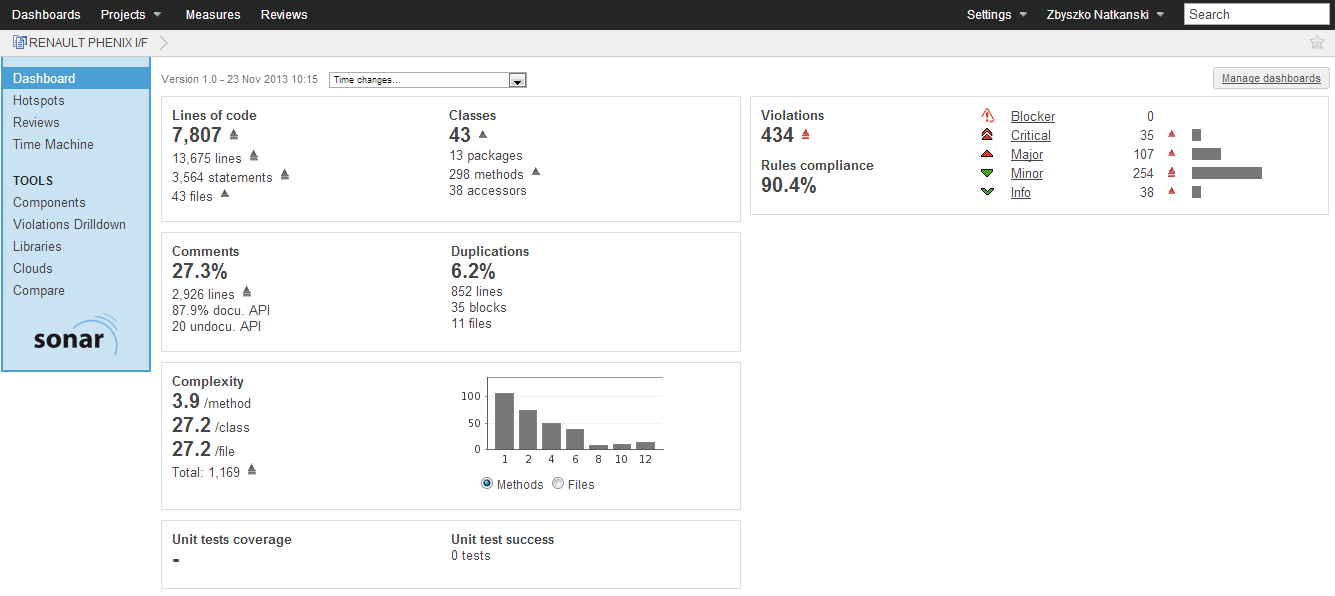
\includegraphics[scale=0.45]{img/sonar2.png} 
	\caption{SonarQube dashboard}		
	\label{fig:sonar1}
\end{figure}


\begin{figure}[h!]
	\centering
	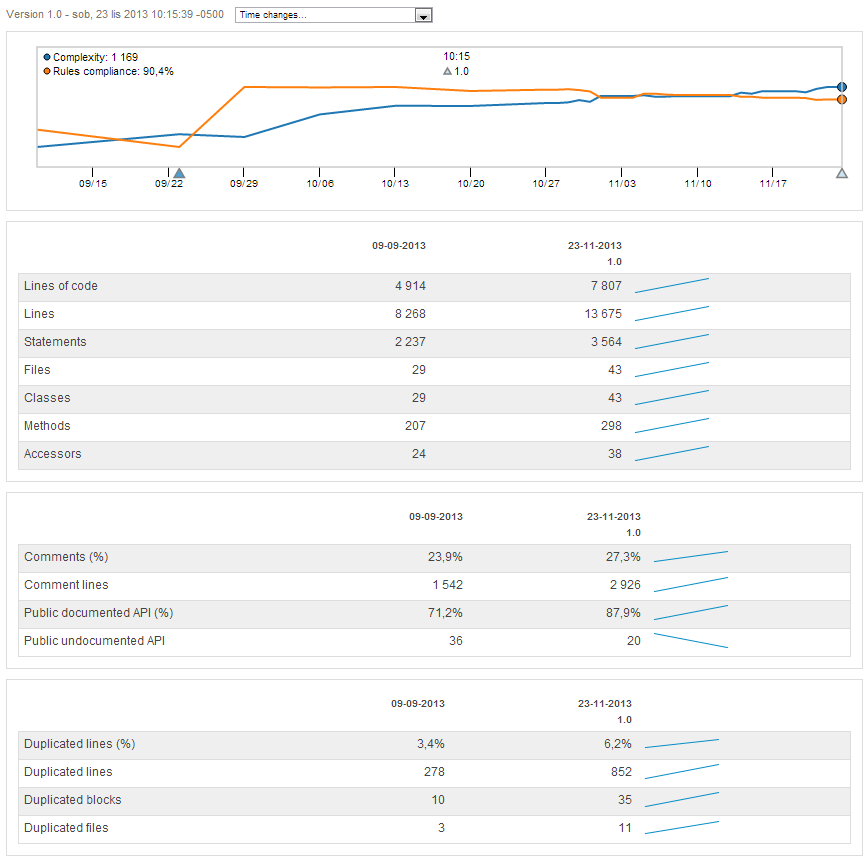
\includegraphics[scale=0.45]{img/sonar4.png} 
	\caption{SonarQube chronological metrics measurement}		
	\label{fig:sonar2}
\end{figure}



%%%%%%%%%%%%%%%%%%%%%%%%%%%%%%%%%%%%%%%%%%%%%%%%%%
\section{SourceMonitor}
SourceMonitor (SM) is measurement metric tool developed by Campwood software. It has graphical user interface and is a freeware closed-source software which runs only on Windows. There are five different views available to display the results: checkpoint, charts, project, details and method view (Figure~\ref{fig:sourcemonitor}). There are multiple supported languages like Visual Basic, HTML, C, C++, Java, and .NET platform languages family. The results of measurements are exported to XML or CSV format files. The implemented metrics are \ac{LoC}, the ratio of methods per class, number of classes and interfaces, Cyclomatic Complexity, the percentage ratio of statements and \ac{LoC} and percentage ratio of commented lines~\cite{indie}.

SourceMonitor is available to download on official website\footnote{SourceMonitor download - \url{http://www.campwoodsw.com/sourcemonitor.html} (access: November 25, 2013).}.

\begin{figure}[h!]
	\centering
	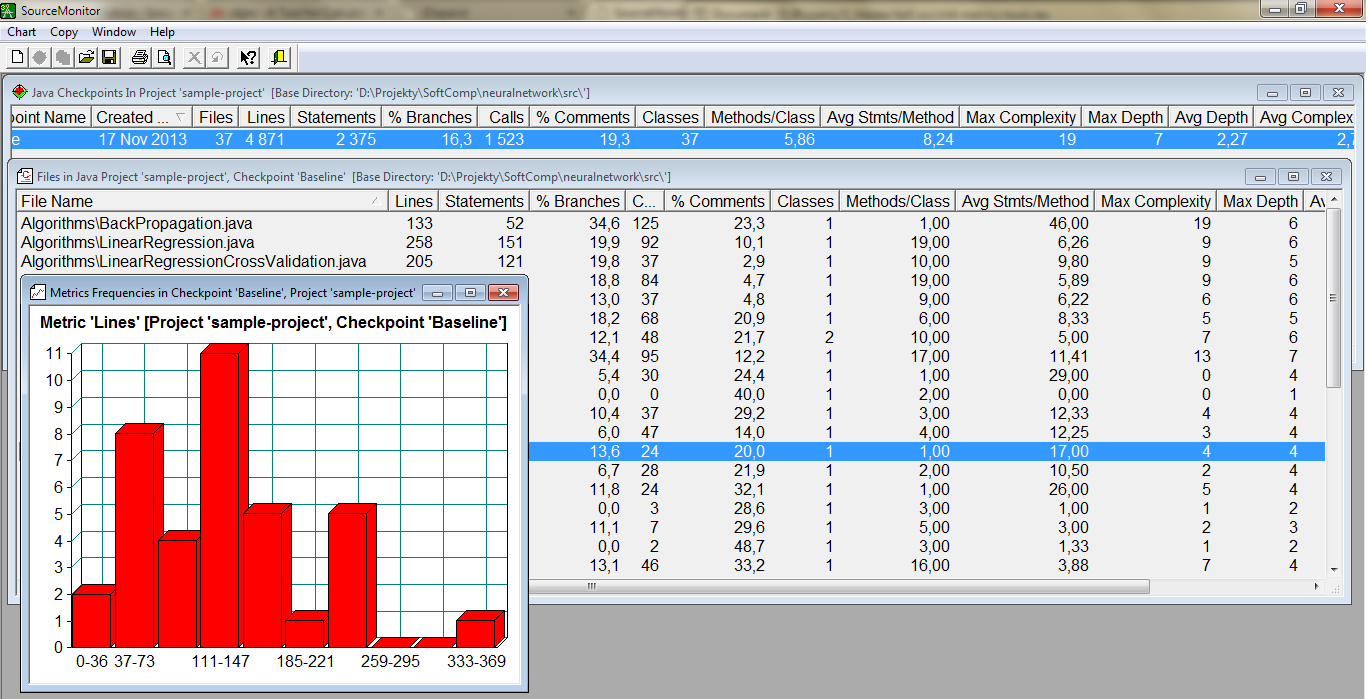
\includegraphics[scale=0.4]{img/sourcemonitor.png} 
	\caption{SourceMonitor metric tool}		
	\label{fig:sourcemonitor}
\end{figure}

%%%%%%%%%%%%%%%%%%%%%%%%%%%%%%%%%%%%%%%%%%%%%%%%%%%%%%%%%%%
\section{Structure Analysis for Java} 
Structure Analysis for Java (STAN) is a tool used to visualizes project design and reports its flaws. It supports in code understanding and measure the quality. STAN offers also set of selected metrics that underline essential aspects of code quality. All faults are clearly visualized what is a key feature for non technical target clients. This tool is used by developers to take care of code quality from the beginning. It could be used by project managers as a tool for monitoring and reporting. 

STAN tool could be downloaded from official website\footnote{STAN official page - \url{http://www.stan4j.com} (access: November 25, 2013).}. It is distributed under the community license option without installing a license key for projects up to 100 classes. There are two variants of product: either standalone application or Eclipse IDE plug-in.

One of the key feature of STAN is computing several metrics. It maps some kinds of artefacts to numbers. The implemented metrics are:

\begin{itemize}
\item size metrics;
\item McCabe's Cyclomatic Complexity;
\item Martin's metrics;
\item \ac{CK metrics}.
\end{itemize}

Metric violations are prioritized  by weighting its rating with the amount of the artifact's underlying code. The results are showed in the violations view (Figure~\ref{fig:stan}). The coupling between classes and packages are presented in coupling view (Figure~\ref{fig:stan2}).

Another interesting feature is customizable reports generation. It gives a detailed lists of metric violations in colourful visualized pie chars and underline bad trends in project design\footnote{Sample report is presented here:~\url{http://stan4j.com/sample-report.html}  (access: November 25, 2013).}~\cite{stan}.

\begin{figure}[h!]
	\centering
	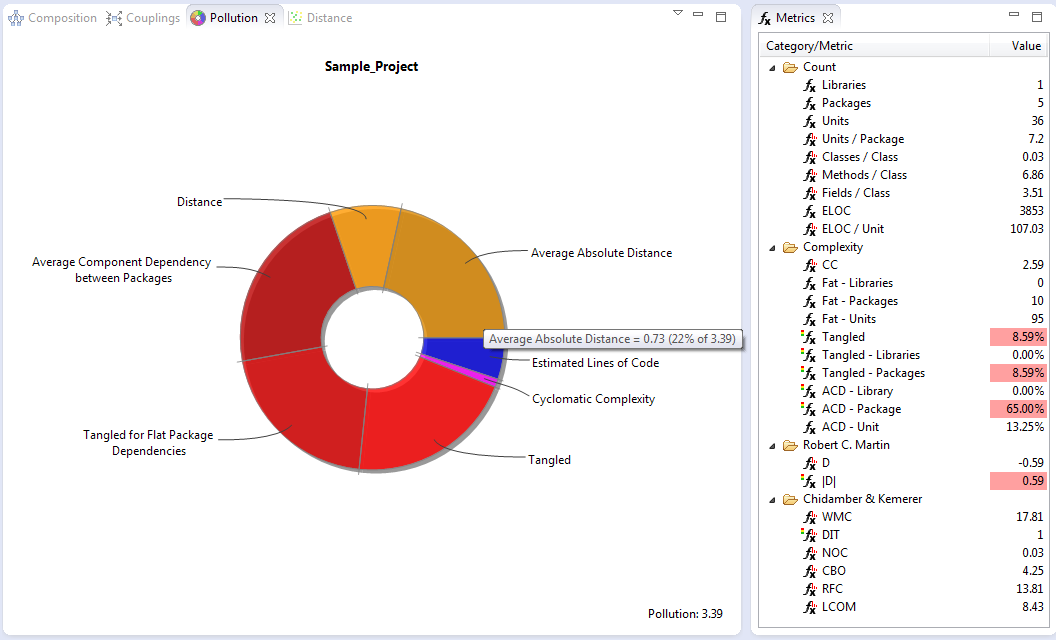
\includegraphics[scale=0.55]{img/stan.png} 
	\caption{STAN: Pollution view}		
	\label{fig:stan}
\end{figure}

\begin{figure}[h!]
	\centering
	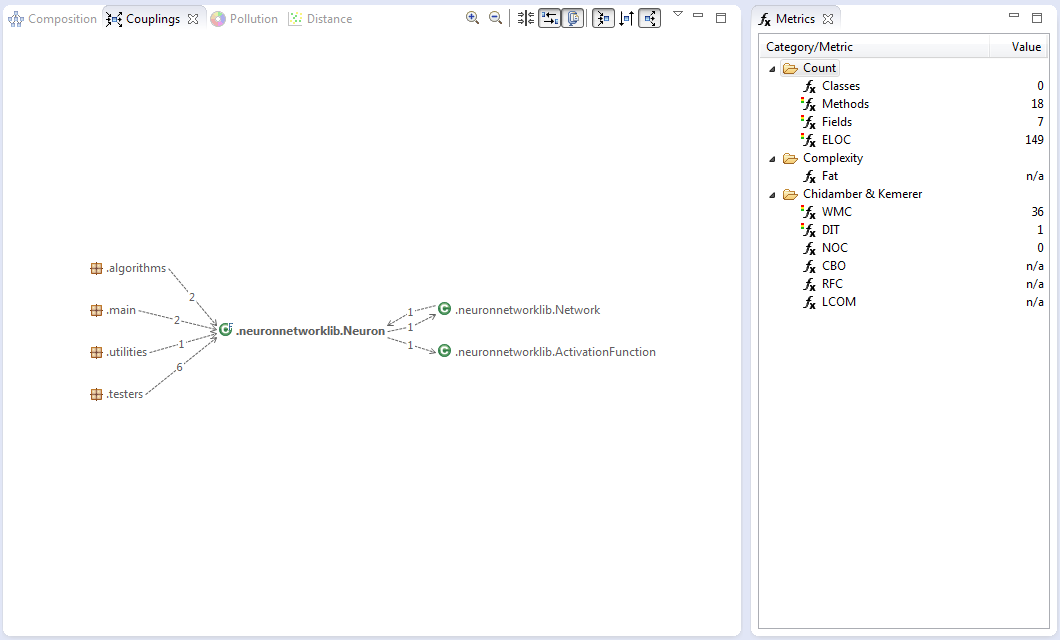
\includegraphics[scale=0.5]{img/stan2.png} 
	\caption{STAN: Coupling view}		
	\label{fig:stan2}
\end{figure}

%%%%%%%%%%%%%%%%%%%%%%%%%%%%%%%%%%%%%%%%%%%%%%%%%%

\section{Summary}

There are much more tools that implements software metrics, however the described set presents its wide range of functionality. Some of them are rather out-of-date (command line applications: C and C++ Code Counter (CCCC) and CKJM -- Chidamber and Kememer Metrics), because it does not visualize the results in tables or charts. What is more, the form of using them is also not comfortable, because it requires additional effort: opening command line, navigating to source files, execution of command and analysing the result in illegible way. Additionally, the number of metrics implemented in these tools is rather poor and low.  

The next group of tools is standalone applications. Nowadays, the \ac{IDE} for software developers is everyday workspace. It is not comfortable to track the quality of provided code in another, separate application, because when the localization of source files changes, there is need to reconfigure the setting of SourceMonitor again. 

In third group, there are plug-ins for Eclipse \ac{IDE}. Currently, the main drawback of Cobertura and Eclipse Metrics Plug-in is fact that they does not provide any visualization in form of charts and number of implemented metrics is also rather low. However, the table view is simple and well-planed, what could encourage to use.

JHawk is a professional tools that provides large set of metrics, however it is a shareware tool. It is not profitable approach, because the same functionality is implemented in another tools that are available for free.      

The last three, not yet mentioned plug-ins, are the leaders of final classification for metrics tools. STAN provides very good visualization on different levels of abstraction and generates histograms for some of metrics. The final report looks very professional and is valuable for project managers, because it emphasizes the parts of project that need to be improved.

RefactorIT provides the largest set of software metrics. It generates the report for every class, package or module. It enables to further analysis of data for overall system. Unfortunately, it is not longer improved and developed, so it is matter of time when it becomes incompatible with the newest versions of Eclipse \ac{IDE}. 

The last one is SonarQube that is currently the best proposition for supporting software metrics. It is a open-source tool that during the last two years had 15 releases. It is commonly used in professional and commercial projects. It offers a full service of code analysis and owning the fact that it is run on web server, the results of analysis is shared with the whole development team.  

\begin{table}[h!]
	\centering
	\begin{tabular}{l}
		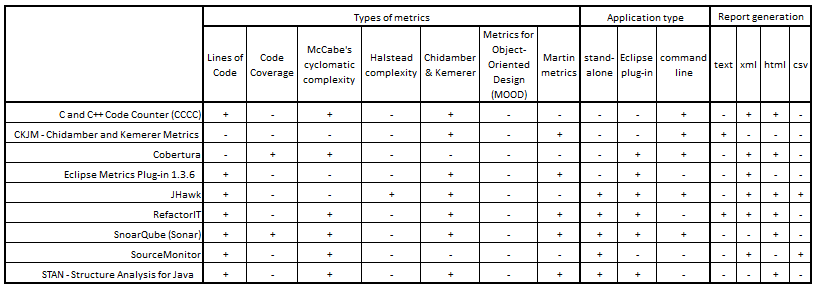
\includegraphics[scale=0.7]{img/tools.png} \\
	\end{tabular}	
		\caption{\textit{Summarize of metrics implemented by set of tools.}}
		\label{tab:summarytools}
\end{table}

The Table~\ref{tab:summarytools} shows the types of metrics implemented in given tool, types of applications and form of measurement results presentation.

Summing up, the developers that want to take care of the code quality and measure it using code metrics have a good set of tools that are available for free.  All described in Chapter~\ref{roz:metrics_theory} metrics are implemented apart from the MOOD metrics. 

\chapter{Practical approach to software metrics} \label{roz:metrics-practic}

\textit{The purpose of this chapter is to use software metrics to improve the quality of code for exemplary academic project. Basing on tools introduced in Chapter~\ref{roz:metrics-tools} (STAN, RefactorIT and JHawk) and metrics described in Chapter~\ref{roz:metrics_theory}, the project is analysed and it is underlined which aspects need improvements.}

\section{Project description}
neural network academic project --- opis

\section{Metrics analysis}
The Figure~\ref{fig:wyniki} presents the results of measurement with use of size metrics, object-oriented metric (\ac{CK metrics}) and package metric (Martin's metrics) for neural network project.  

\begin{figure}[h!]
	\centering
	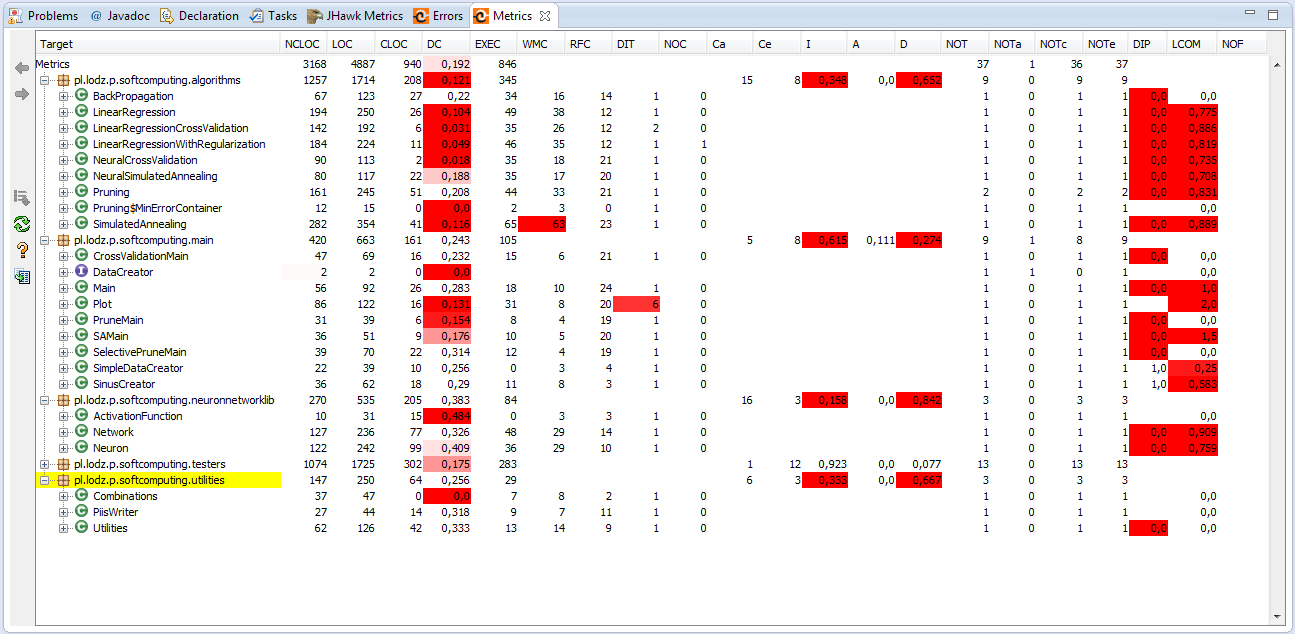
\includegraphics[scale=0.45]{img/wyniki-refactorIT.png} 
	\caption{The results for neural network project generated by RefactorIT.}		
	\label{fig:wyniki}
\end{figure}

\subsubsection*{Size metrics}
The Lines of Code (\ac{LoC}) metric in RefactorIT does not take into account comments, empty lines and imports. The non-commented lines of code (\ac{NCLOC}) counts the lines that are not comments or empty lines. The commented lines of code (\ac{CLOC}) informs how many lines contains comments or Java docs. The executable statements (\ac{EXEC} indicates the lines that are executable statements. 

The main function of already mentioned metrics and these from NOT--family metrics (number of types (\ac{NOT}), number of abstract types (\ac{NOTa}), number of concrete types (\ac{NOTc}), number of exported types (\ac{NOTe})) is to inform about the size of project. The greater values are, the more effort has been taken to prepare the implementation. In this case, any values exceeding is predicted. 

The density of comments (\ac{DC}) metric determines a density value of how commented the code is. The red background indicated that there are classes which are not enough commented. In other words, there are no Java docs provided for every class, method or attribute in given package.

\subsubsection*{Object-oriented metrics}
The next group studied by RefactorIT tool is \ac{CK metrics}. According to NASA publication \cite{nasa} that made the research about object-oriented projects. In complex system, 60\% of class have \ac{WMC} values smaller than 20, about 36\% between 20 and 100, and only 4\% of class have \ac{WMC} greater than 100. In this case, the neural network project has only one class (\texttt{SimulatedAnnealing}) that exceeds desired value. It means that it is the most complex class and it needs to be reimplemented. The difference in compare to rest of classes is really high. 

The greater \ac{RFC} value is, the more complex and functional class is. It causes problems in testing and maintenance. Analysing \ac{RFC} values for neutral network project, it could be stated that the most complex are classes which values exceed 20. They are usually in \textit{pl.lodz.p.softcomputing.algorithms} package what proves the definition of \ac{RFC}.       

In case of \ac{DIT} metric, the greater number of class that given child class inherits, the deeper degree of complexity is. It increases the cost of maintenance, so the class chain that leads to \texttt{Plot} class should be shorten. 

The next from \ac{CK metrics} set is \ac{LCOM} metric, but more precisely LCOM2 metric. The results should be returned in interval between 0 and 1. The smallest values are the better. As it could be observed, the area of improvements in that case is very wide. It indicates lack of cohesion inside the methods.  

The results of \ac{NOC} metric shows that inheritance is poorly used in neural network project which could lead to code duplication. The \ac{CBO} metric is not implemented in RefactorIT.

\subsubsection*{Martin's metric}
The Martin's metrics that into consideration the packages inside the neural network project. The upper limit for values of efferent coupling (\ac{Ce}) is 20. Neither of packages exceed it. The same situation is with afferent coupling (\ac{Ca}), however the tolerance for \ac{Ca} is equal even to 500. 

The abstractness (\ac{A}) calculates the relationship between number of interfaces and classes within the package. Only for a one package this ratio has been calculated (\textit{pl.lodz.p.soft\-com\-pu\-ting.main}). The resultant value means that the package is open to changes in implementation.

The instability (\ac{I}) calculated the effort needed to change a package without impacting others. The stability of the package is defined in range 0.0 to 0.3. In this case of \textit{pl.lodz.p.soft\-com\-pu\-ting.al\-go\-rithms, pl.lodz.p.soft\-com\-pu\-ting.neu\-ron\-net\-work\-lib} and \textit{pl.\-lodz.\-p.\-soft\-com\-pu\-ting.u\-ti\-li\-ties} packages could be stated that are or are closed to be treated as stable. The packages: \textit{pl.lodz.p.soft\-com\-pu\-ting.main} and \textit{pl.lodz.p.soft\-com\-pu\-ting.tes\-ters} are considered as unstable or as close to be unstable packages.

The last from Martin's metrics set is distance from the main square (\ac{D}). The values close to 0 are desirable ones. Any package that is not close to zero is considered as unbalanced and need to be reimplemented to be less sensitive to changes~\cite{martin}. The only acceptable is value for \textit{pl.lodz.p.soft\-com\-pu\-ting.tes\-ters} package. The values for the rest of packages are not acceptable. 

\subsubsection*{Halstead complexity metrics}
The Halstead complexity metrics are implemented only in JHawk plug-in. The shareware version of JHawk enables to calculate four of metrics: program length, program volume difficulty error proneness and effort to implement but only on package or class level. It is not possible to generates those results for the whole project in freeware version. The Figure~\ref{fig:jhawk3} presents the results for  \textit{pl.lodz.p.soft\-com\-pu\-ting.al\-go\-rithms} package. 

\begin{figure}[h!]
	\centering
	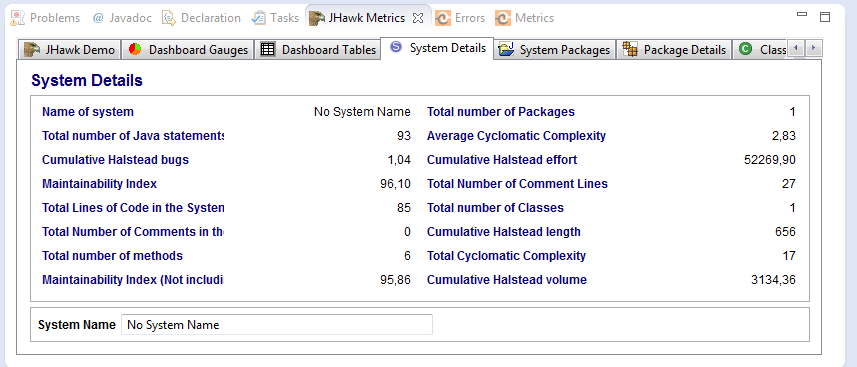
\includegraphics[scale=0.7]{img/jhawk3.png}  
	\caption{Results of Halstead metrics generated by JHawk plug-in.}		
	\label{fig:jhawk3}
\end{figure}

The results of program level and time to implement metrics could be very easily derived from provided formulas described in section~\ref{sec:halstead}. 

For program level (L):
\[L=\frac { 1 }{ 1,04 } \approx 0,96\]

For time to implement (T):
\[T=\frac { 52699,9 }{ 18 } \approx 2903,88\quad seconds\]

Basing on the results could be stated that implementation of researched package requires 48~minutes and 24~seconds. The obtained result is only theoretical and does not take into consideration any external factors.  

\subsubsection*{McCabe's cyclomatic complexity}


\section{Summary}
rozwijac dziedziczenie i go uzyc

wiecej komentarzy

cohesion

paczki słabo - stable vs unstable   oraz distance

halstead smieszne i trywialne
%conclusion
\chapter{Conclusions} \label{roz:conclusion}

\section{Final remarks}
Software engineers: design architects, developers and project managers are likely to rely on scientific results, especially those research on software quality. That s why, metrics should be reliable because they are used to measure if following components of a system keep the quality or they are used to predict effort for maintenance activity and identify system components that need particular attention. 

From one side, software metrics verify the laws and rules of structural and object--oriented programming, so they are a great support for good coding practise, but from the other side they are not developed and research commonly by academic and professional development environment. That is why, some of metrics assumptions are out of date and does not take into consideration the newest aspects of modern programming.

Software engineers are able to rely on the tools implementing these metrics. They allow to quantify the software quality and deliver information needed to take a decisions during designing and implementing process. However, the threshold values defined in these tools are not based on any theoretical and practical research so it should be treated with reserve. The main advantage of metrics tools is a fact that they are available for free in most of the cases. The leader of final classification is definitely SonarQube that is commonly used in many professional and commercial projects. The range of provided metrics is quite impressive and it is still developed. 

From the scientific point of view, the results of measurement using described tools are strongly dependent on the implementing tools, so a validation supports the applicability of some metrics as implemented by the given tool. 

The practical approach described in Chapter~\ref{roz:metrics-practic} shows how software metrics could be used in arbitrary programming project. The results of measurement show areas of increased risk of faults appearance and potential maintenance problem. However, it was mentioned that the threshold values could be freely changed and it does not mean that developers should refactor its code. 

Undoubtedly software metrics are one of the first instruments available to project development management, because they are early indicators to risk-prone issues. In context of each software project, the project managers are able to formulate their own metrics and leading metrics tool in order to address company's unique strategic goals, priorities and clients custom needs and expectations to fully satisfy their requirements. 

\section{Further development}
This thesis enhances the set of commonly used software metrics and presents the advantages and disadvantages of metrics tools. Like most of research, this study has several limitations, because it covers only a subset of metrics and tools. This research needs to be further extended with wider set of software metrics to evaluate many more measurements and comparison.

Using metrics in practise is not a easy approach, because it requires an experience and developing own skills to provide a good software products. One of the further development for software metrics  is to determine generic and unique threshold values characteristic in given programming language or environment. Such approach opens an opportunity to define own, well-designed and described metrics.

Another further consideration is developing set of tools that implements already existing or newly defined metrics. Currently, many tools are either out of date or not developed any more. This is a kind of market that business niche has created.   

The last consideration that is not appreciated in context of software metrics is fact that they are a perfect \textit{tool} to teach the good coding practise and show the area of commonly made mistakes in given programming language.
                
%------------------------------------------------------------
% bibliografia          
                \newpage
                \phantomsection \label{bib}
                \addcontentsline{toc}{chapter}{Bibliography}
                \begin{thebibliography}{100}

\subsection*{Books}

	\bibitem{alain} Abran A., {\em Software Metrics and Software Metrology}, IEEE Computer Society, Los Alamitos, 2010.	
	
	\bibitem{graph} Berge C., {\em Theory of Graphs}, Dover Publications, 2001. 
	
	\bibitem{booch} Booch G., {\em Object-Oriented Analysis and Design with Applications}, Addison-Wesley, 2007.
	
	\bibitem{rigorous} Fenton N., Pfleeger S., {\em Software Metrics - A Rigorous And Practical Approach}, PWS Publishing Company, Boston, 1997.
	
	\bibitem{metrics} Kan S., {\em Metrics and Models in Software Quality Engineering}, Addison Wesley, 2002.

	\bibitem{moodbook} Sarker M., {\em An overview of Object Oriented Design Metrics}, Department of Computer Science at Sweden Umea University, Umea, 2005.
		
	\bibitem{SCJP} Sierra K., Bates B., {\em Sun Certified Programmer for Java 6}, Mc Graw Hill, 2008.
	
\subsection*{Online documents}

	\bibitem{complexity1} Aivosto.com, {\em Complexity metrics}, [access: November 9, 2013]. \\ Available at: \url{http://www.aivosto.com/project/help/pm-complexity.html}. 
	
	\bibitem{directedGraph} Algorithms Overview, {\em A directed graphs}, [access: November 9, 2013].\\  Available at: \url{http://algs4.cs.princeton.edu/42directed/}.

\bibitem{indie} Chawla M. K., Chhabra I., {\em }, Department of Computer Science Department in Panjab University in Chandigarh (India), [access: November 17,2013]. Available at: \url{http://tnijurl.com/f97365e79185/}.

	\bibitem{coverage1} Cornett S., {\em Code Coverage Analysis}, [access: November 3, 2013]. Available at: \url{http://www.bullseye.com/coverage.html}.

	\bibitem{ISO9126} ISO 9126 Software Quality Characteristics,{\em An overview of the ISO 9126-1 software quality model definition, with an explanation of the major characteristics}, [access: November 26, 2013]. Available at: \url{http://www.sqa.net/iso9126.html}.

	\bibitem{JavaDoc} Java Tutorials, The, {\em Polymorphism}, [access: October 7, 2013]. Available at: \\ \url{http://docs.oracle.com/javase/tutorial/java/IandI/polymorphism.html}.	
	
	\bibitem{coverage2} Johnson P., {\em Testing and Code Coverage}, [access: November 3, 2013]. Available at: \url{http://pjcj.net/testing_and_code_coverage/paper.html}.

	\bibitem{vaxjo} Lincke R, Lundberg J., Lowe W., {\em Comparing Software Metrics Tools}, School of Mathematics and Systems Engineering in Vaxjo University in Sweden, [access: November 17, 2013]. Available at: \url{http://www.cs.umd.edu/~pugh/ISSTA08/issta2008/p131.pdf}.
 
	\bibitem{cccc1} Littlefair T., {\em CCCC. User Guide}, [access: November 17, 2013]. Available at: \url{http://www.stderr.org/doc/cccc/CCCC\%20User\%20Guide.html}. 

	\bibitem{stan} Odysseus Software GmbH, {\em STAN – Structure Analysis for Java}, [access: November 16, 2013]. Available at: \url{http://stan4j.com/papers/stan-whitepaper.pdf}. 
 	
	\bibitem{martin} Martin R. {\em OO Design Quality Metrics. An Analysis of Dependencies}, [access: November 11, 2013]. Available at: \url{http://www.cin.ufpe.br/~alt/mestrado/oodmetrc.pdf}.
	
	\bibitem{nasa} Rosenberg L., {\em Applying and Interpreting Object Oriented Metrics}, Software Assurance Technology Center (SATC) in NASA, [access: November 9, 2013]. Available at: \url{http://www.literateprogramming.com/ooapply.pdf}.
 
\end{thebibliography}

%------------------------------------------------------------
%spis rysunkow
                \newpage
                \phantomsection \label{listoffig}
                \addcontentsline{toc}{chapter}{List of Figures}
                \listoffigures
%------------------------------------------------------------
%spis tabel
                \newpage
                \phantomsection \label{listoftab}
                \addcontentsline{toc}{chapter}{List of Tables}
                \listoftables
                
%------------------------------------------------------------
%skroty
                \newpage
                \phantomsection \label{acronyms}
                \addcontentsline{toc}{chapter}{Acronyms}
                \chapter*{List of Acronyms}
\begin{acronym}
\acro{A}{Abstractness}
\acro{AHF}{Attribute Hiding Factor}
\acro{AIF}{Attribute Inheritance Factor}
\acro{Ca}{Afferent Coupling}
\acro{CAD}{Computer Aided Design}
\acro{CBO}{Coupling Between Objects}
\acro{CC}{Cyclomatic Complexity}
\acro{Ce}{Efferent Coupling}
\acro{CF}{Coupling Factor}
\acro{CK metrics}{Chidamber \& Kemerer metrics}
\acro{CLOC}{Comment Lines of Code}
\acro{COM}{Lines of Comments}
\acro{CYC}{Cyclic Dependencies}
\acro{D}{Distance from the Main Sequence}
\acro{DC}{Density of Comments}
\acro{DCYC}{Direct Cyclic Dependencies}
\acro{DIP}{Dependency Inversion Principle}
\acro{DIT}{Depth of Inheritance Tree}
\acro{EP}{Encapsulation Principle}
\acro{EXEC}{Executable Statements}
\acro{I}{Instability}
\acro{IDE}{Integrated Development Environment}
\acro{LC}{Lines of code per line of comment}
\acro{LCOM}{Lack of Cohesion in Methods}
\acro{LLoC}{Logical Lines of Code}
\acro{LoC}{Lines of Code}
\acro{LSP}{Limited Size Principle}
\acro{MC}{Cyclomatic Complexity per line of comment}
\acro{MHF}{Method Hiding Factor}
\acro{MIF}{Method Inheritance Factor}
\acro{MOOD}{Metrics for Object-Oriented Design}
\acro{MQ}{Modularization Quality}
\acro{NCLOC}{Non-Comment Lines of Code}
\acro{NOA}{Number Of Attributes}
\acro{NOC}{Number of Children of Class}
\acro{NOF}{Number Of Fields }
\acro{NOM}{Number of Modules}
\acro{NOT}{Number of Types}
\acro{NOTa}{Number of Abstract Types}
\acro{NOTc}{Number of Concrete Types}
\acro{NOTe}{Number of Exported Types}
\acro{NP}{Number of Parameters}
\acro{PF}{Polymorphism Factor}
\acro{RFC}{Response for a Class}
\acro{SLoC}{Source Lines of Code}
\acro{WMC}{Weighted Methods per Class}

\end{acronym}                 
%------------------------------------------------------------

\end{document}
